\documentclass[lettersize,journal]{IEEEtran}
\usepackage{amsmath,amsfonts}
\usepackage{algorithmic}
\usepackage{algorithm}
\usepackage{array}
\usepackage[caption=false,font=normalsize,labelfont=sf,textfont=sf]{subfig}
\usepackage{textcomp}
\usepackage{stfloats}
\usepackage{url}
\usepackage{verbatim}
\usepackage{graphicx}
\usepackage{cite}


% ==== MJ thing ==== %
\usepackage{amsthm}
\usepackage{amssymb}
\usepackage{caption}
\usepackage{booktabs}
\usepackage{yhmath}
\usepackage{multirow}
\usepackage{todonotes}
\usepackage{subcaption} % Must be BEFORE hyperref/cleveref
\usepackage{cite}       % Must be BEFORE hyperref/cleveref
\usepackage{mathtools}  % Must be BEFORE hyperref/cleveref

\usepackage{hyperref}   % Load 2nd to last
\usepackage{cleveref}   % MUST BE LOADED ABSOLUTELY LAST

\captionsetup[figure]{font=footnotesize}
\captionsetup[table]{font=footnotesize}

\newcommand{\mc}{\mathcal}
\newcommand{\mb}{\mathbb}
\newcommand{\mf}{\mathbf}
\newcommand{\red}[1]{{\color{red}#1}}
\newcommand{\blue}[1]{{\color{blue}#1}}
\newcommand{\alg}{$\text{C}^2\text{RL}$}

\newtheorem{assumption}{Assumption}
\newtheorem{remark}{Remark}
\newtheorem{lemma}{Lemma}
\newtheorem{example}{Example}
\newtheorem{theorem}{Theorem}
\newtheorem{definition}{Definition}
\newtheorem{proposition}{Proposition}
\newtheorem{corollary}{Corollary}

% Optional but highly recommended: Explicitly tell cleveref how to name your custom environments
\crefname{assumption}{Assumption}{Assumptions}
\crefname{lemma}{Lemma}{Lemmas}
\crefname{theorem}{Theorem}{Theorems}
\crefname{proposition}{Proposition}{Propositions}
\DeclareMathOperator*{\argmax}{argmax}
\DeclareMathOperator*{\argmin}{argmin}


\hyphenation{op-tical net-works semi-conduc-tor IEEE-Xplore}
% updated with editorial comments 8/9/2021

\begin{document}

\title{State-Dependent Contraction Bounds for Reinforcement Learning-Based Nonlinear Control}

\author{Anonymous Authors
        % <-this % stops a space
\thanks{This manuscript is submitted for double-blind review.}% <-this % stops a space
}


% \author{Minjae Cho, Hiroyasu Tsukamoto, and Huy T. Tran
% % \thanks{This work was supported by the relevant funding agencies.}
% \thanks{M. Cho, H. Tsukamoto, and H. T. Tran are with the Department of Aerospace Engineering, The Grainger College of Engineering, University of Illinois Urbana-Champaign, Urbana, IL 61801 USA (e-mail: \{minjae5, hiroyasu, huytran1\}@illinois.edu.}}



% The paper headers
\markboth{Journal of \LaTeX\ Class Files,~Vol.~14, No.~8, August~2021}%
{Shell \MakeLowercase{\textit{et al.}}: A Sample Article Using IEEEtran.cls for IEEE Journals}

% \IEEEpubid{0000--0000/00\$00.00~\copyright~2021 IEEE}
% Remember, if you use this you must call \IEEEpubidadjcol in the second
% column for its text to clear the IEEEpubid mark.

\maketitle

\begin{abstract}
While proving uniform contraction bounds is now a tractable convex optimization problem, analyzing state-dependent rates to establish tighter contraction bounds remains a long-standing challenge. 
In this work, we provide the conditions on system dynamics necessary for the existence of state-dependent contraction rates. 
We propose a theoretical reinforcement learning (RL) framework that offers a natural pathway to leverage higher contraction rates using its optimality. 
Specifically, for RL algorithms designed to minimize cumulative tracking errors defined by uniform-rate contraction metrics, we formally establish state-dependent contraction bounds that decay at the highest feasible contraction rate at each state.
% The derived bounds capture two phenomena driven by RL optimality: transient overshoot, which arises from prioritizing future returns at the expense of immediate errors, and a state-dependent contraction rate, where the policy maximizes contraction speed when the dynamics allow. 
% In the worst case, the state-dependent contraction rate gracefully reduces to a uniform contraction rate. 
% To better understand this optimality-driven behavior, we empirically investigate how the discount factor---which dictates the degree of optimality of the RL algorithms---modulates the trade-off between transient overshoot and sustained faster state-dependent contraction.
\end{abstract}

\begin{IEEEkeywords}
Article submission, IEEE, IEEEtran, journal, \LaTeX, paper, template, typesetting.
\end{IEEEkeywords}

\section{Introduction}
\IEEEPARstart{T}{he} existence of contraction metrics \cite{LOHMILLER1998683}---Riemannian metrics under which any two trajectories of a dynamical system converge exponentially---certifies incremental exponential stability (IES).
For control-affine systems, the contraction metrics are used to synthesize control laws that render the closed-loop systems contracting \cite{manchester2017control}.
Such synthesis, however, is often conservative, as the contraction condition is imposed with a single rate that must hold uniformly across the state space.
Thus, the resulting controller is limited when a subset of states allows for higher contraction rates, as it only certifies a much lower global rate.

We show that reinforcement learning (RL)---minimizing the cumulative tracking error defined by a contraction metric---resolves this conservatism through its optimality.
Specifically, we propose state-dependent contraction bounds of optimal policies trained by the RL algorithms and show the bounds decay at the highest feasible rate at that state, while the optimal policies were optimized using contraction metrics that certify a slower uniform rate.
% Crucially, it is optimality alone---not a state-dependent redesign of the metric---that recovers the local rate: the metric is certified with a single uniform rate, and the state-dependence emerges entirely from the optimized policy.
However, we note that this benefit comes at a cost, as it requires a larger overshoot margin.

To establish this, we proceed in two steps.
First, we characterize when a state-dependent contraction rate exists---that is, when the highest certifiable rate genuinely varies across the state space rather than remaining fixed.
Second, for systems in this regime, we derive state-dependent contraction bounds for RL-optimized policies: at each state, the tracking error decays at the highest feasible rate for that state, even though the underlying metric is certified with only a uniform contraction rate.
In the worst case, the bound reduces gracefully to that uniform rate.
% The same analysis exposes a transient overshoot induced by optimality, in which the policy tolerates larger immediate error in exchange for smaller error over the horizon.

\begin{figure}[t]
    \centering
    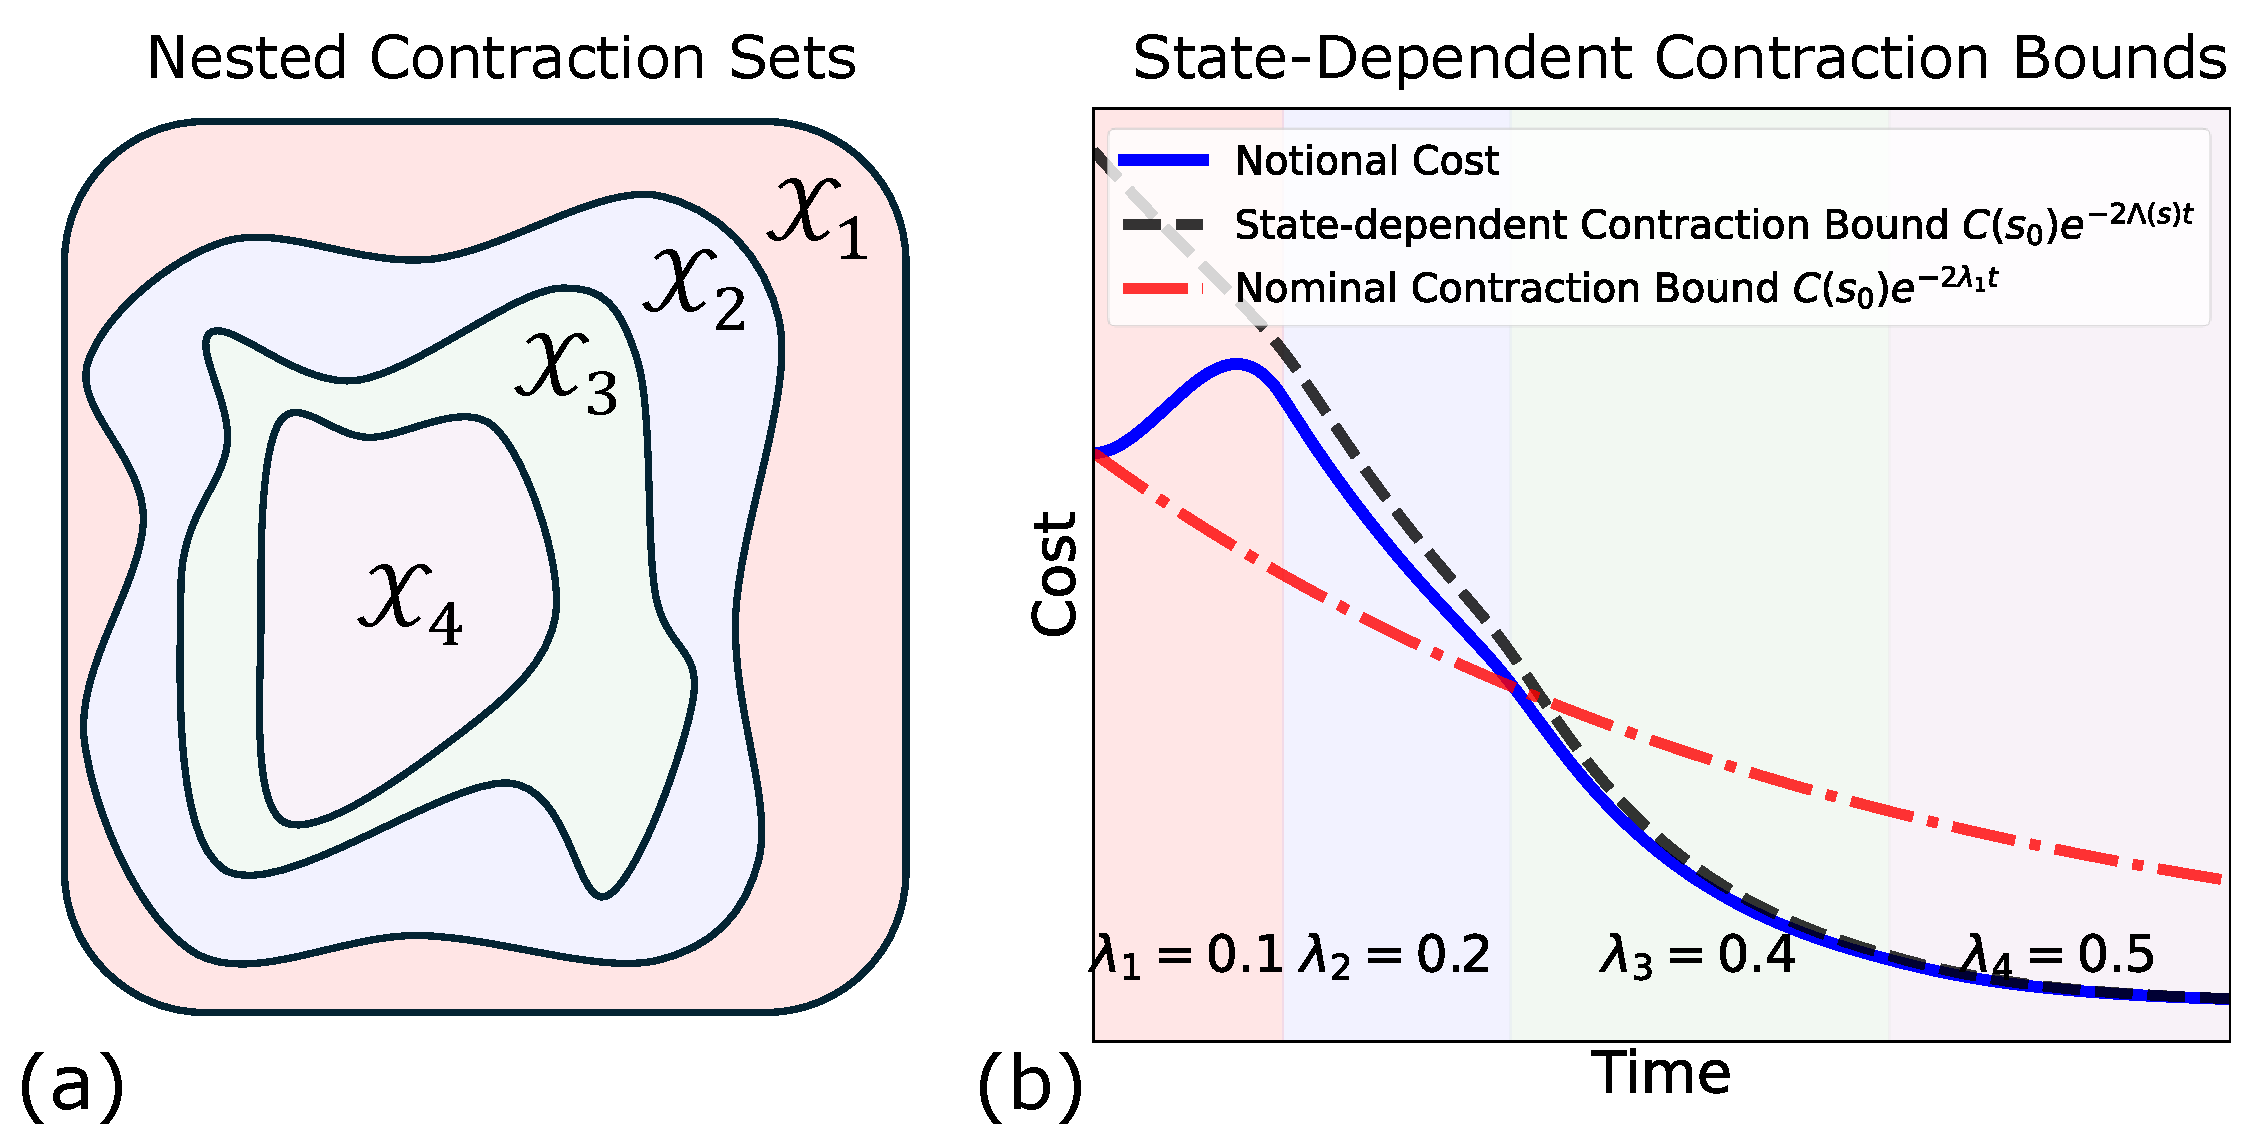
\includegraphics[width=0.99\linewidth]{fig/Notional_contraction_plot.pdf}
    \caption{(a) Nested contraction sets, where each successive subset guarantees a higher contraction rate. (b) An illustrative error (cost) plot showing how state-dependent contraction takes place across the subsets in (a). It highlights that progressively faster contraction rates become available as the system transitions to state subsets where higher contraction is available.}
    \label{fig:notional_diagram}
\end{figure}



%%%%%%%%%%%%%%%%%%%%%%%%%%%%%%%%%%%%%%%%%%%%%%%%%%%%%%%%%
\section{Preliminaries}\label{sec:preliminaries}
%%%%%%%%%%%%%%%%%%%%%%%%%%%%%%%%%%%%%%%%%%%%%%%%%%%%%%%%%

\subsection{Dynamical System and Contraction Metrics}
In this work, we consider control-affine nonlinear dynamical systems of the form:
\begin{equation}\label{eqn:control_affine_system}
    \dot{x} = f(x) + B(x)u,
\end{equation}
where $x \in \mathcal{X} \subset \mathbb{R}^n$ is the $n$-dimensional state, $u \in \mathcal{U} \subset \mathbb{R}^m$ is the $m$-dimensional control input, $f: \mc{X} \rightarrow \mb{R}^n$ represents the drift dynamics, and $B: \mc{X} \rightarrow \mb{R}^n \times \mb{R}^n$ is the actuation matrix function. 

Solution trajectories of \Cref{eqn:control_affine_system} contract toward one another if there exists a uniformly bounded, positive-definite contraction metric $M(x)$ satisfying $\underline{m}I \preceq M(x) \preceq \bar{m}I$ for $0 < \underline{m} \leq \overline{m} < \infty$, along with the following condition:
\begin{equation}\label{eqn:contraction_condition}
    \dot{M} + \widehat{M(A + BK)} + 2 \lambda M \preceq 0,
\end{equation}
where the arguments are omitted for brevity. Here, $\lambda > 0$ defines the contraction rate, and the hat operator denotes the symmetric sum ($\widehat{A} \coloneq A + A^\top$). The matrix $A(x, u) = \frac{\partial f}{\partial x} + \sum_{i=1}^m u_i \frac{\partial b_i}{\partial x}$ is the Jacobian of the system dynamics, and $K(x, t) = \frac{\partial \pi_c}{\partial x}$ represents the differential feedback gain of the baseline policy.

\subsection{Reinforcement Learning}
% Reinforcement learning (RL) provides a framework for solving optimal control problems through environmental interaction. 
We formulate the nonlinear control problem as a discounted Markov decision process (MDP) \cite{puterman2014markov}, defined by the tuple $(\mathcal{S}, \mathcal{U}, P, R, \gamma)$, where $\mathcal{S}$ and $\mathcal{U}$ denote the state and control spaces, respectively. 
The environment dynamics are characterized by the transition probability density $P(s' \mid s, u): \mathcal{S} \times \mathcal{U} \times \mathcal{S} \rightarrow [0, \infty)$, while $R(s, u, s') : \mathcal{S} \times \mathcal{U} \times \mathcal{S} \rightarrow [0, R_{\max}]$ represents the reward function, and $\gamma \in [0,1)$ is the discount factor. 
The value function $V_{R}^{\pi}(s)$ and the overall performance $J_{R}(\pi)$ under policy $\pi$ are defined as:
\begin{align}
    V_{R}^{\pi}(s) & \coloneq \mathbb{E}_\pi \left[ \sum_{k=0}^{\infty} \gamma^k R(s_{t + k}, u_{t+k}) \mid s_t = s \right], \label{eqn:reward_value_function}\\
    J_{R}(\pi) & \coloneq \mathbb{E}_{s_0 \sim d_0}\left[ V_{R}^{\pi}(s_0) \right], \label{eqn:reward_performance}
\end{align}
where $d_0$ denotes the initial state distribution. 
The deterministic optimal policy $\pi^\star$ is then given by:
\begin{equation}\label{eqn:discounted_optimal_policy}
    \pi^\star \coloneq \argmax_\pi J_{R}(\pi).
\end{equation}


\section{State-Dependent Contraction Analysis}\label{sec:state_dependent_rate}
We characterize when a control-affine system admits a state-dependent
contraction rate and reduce this question to a single, checkable condition on
the pair $(A(x),B(x))$, where $A(x)\coloneq\partial f/\partial x$.

For a contraction-feasible system, let the per-state optimal certified rate be defined as follows:
\begin{equation}\label{eq:lambda_star_x}
    \lambda^*(x) := \sup \bigl\{ \lambda : \mathcal{P}(\{x\})\ \text{is feasible} \bigr\}.
\end{equation}

\begin{definition}[Contraction-Rate Classes]\label{def:classes}
The dynamics are \emph{uniform-rate} (Class~I) if $\lambda^*(\cdot)$ is constant
on $\mathcal{X}$, and \emph{state-dependent} (Class~II) if
$\lambda^*(x_1)\neq\lambda^*(x_2)$ for some $x_1,x_2\in\mathcal{X}$.
\end{definition}

The certification problem $\mathcal{P}(\{x\})$ is invariant under the orthogonal
congruence $\bar W\mapsto T\bar W T^\top$, $T\in O(n)$. Hence $\lambda^*(x)$
depends on $(A(x),B(x))$ only through its orthogonal-equivalence class, which
yields the following test.

\begin{proposition}[Orthogonal Reduction Test]\label{prop:orthogonal_test}
If there exist a map $T:\mathcal{X}\rightarrow O(n)$ and a fixed pair
$(A_0,B_0)$ such that
\begin{equation}\label{eq:orthogonal_reduction}
    T(x)A(x)T(x)^\top=A_0, \; T(x)B(x)B(x)^\top T(x)^\top = B_0B_0^\top
\end{equation}
for all $x\in\mathcal{X}$, then $\lambda^*(x)=\lambda_0^*$ for all $x\in\mathcal{X}$, where $\lambda_0^*$ is the optimal certified rate of $(A_0,B_0)$; the rate is uniform. 
Consequently, a state-dependent rate can arise only when no such reduction exists.
\end{proposition}

% \begin{proof}
%     Fix $x \in X$ and let $T = T(x)$. The congruence transformation $\bar{W} \mapsto T^\top \bar{W}_0 T$ is a bijection between feasible points of $\mathcal{P}(\{x_0\})$ and $\mathcal{P}(\{x\})$.
%     Substituting $\bar{W} = T^\top \bar{W}_0 T$ and utilizing $A = T^\top A_0 T$, $BB^\top = T^\top B_0 B_0^\top T$, and $T^\top T = I$, the terms of \eqref{eq:C1} transform cleanly:
%     \begin{equation}
%         A\bar{W} + \bar{W}A^\top = T^\top(A_0\bar{W}_0 + \bar{W}_0 A_0^\top)T, \quad \frac{1}{dt}(\bar{W} - I) = T^\top \frac{1}{dt}(\bar{W}_0 - I)T
%     \end{equation}
%     Orthogonal congruence preserves the PSD ordering, eigenvalues (satisfying \eqref{eq:C2}), and scalar dependencies \eqref{eq:C3}. Thus, feasibility is identical at all $x$, making $\lambda^*$ uniform.
% \end{proof}

\begin{proof}[Proof Sketch]
Under \eqref{eq:orthogonal_reduction}, the congruence $\bar W\mapsto T(x)\bar W T(x)^\top$ (with $T(x)^\top T(x)=I$) maps $\mathcal{P}(\{x\})$ onto the fixed problem for $(A_0,B_0)$; orthogonal invariance of the underlying condition then gives identical feasibility at every $x$, so $\lambda^*(\cdot)\coloneq \lambda_0^*$.
\end{proof}

\Cref{prop:orthogonal_test} acts as a structural screen. If the pairs reduce to a common $(A_0,B_0)$, the system is uniform-rate and no per-state analysis is needed; if the reduction fails, the certified rate may vary over the state space.

% \begin{remark}[Implications for synthesis]
% \label{rem:synthesis}
% When the structural hypothesis of \Cref{prop:orthogonal_classI} fails, the
% certified rate generally varies over $\mathcal{X}$ (Class~II). In this regime,
% certifying a single uniform rate $\lambda\leq\inf_{x}\lambda^*(x)$---as the
% CV-STEM program of \Cref{subsec:rate_discovery} does---is conservative wherever
% $\lambda^*(x)$ exceeds this infimum, since the resulting feedback
% under-exploits the locally available contraction. A state-dependent metric that
% tracks $\lambda^*(x)$ pointwise recovers this margin, at the expense of a
% spatially varying geodesic feedback gain. For Class~I plants, by contrast, a
% single metric attains the best certifiable rate everywhere and no
% gain-scheduling is warranted.
% \end{remark}

\subsection{Discovery of the contraction rate}
\label{subsec:rate_discovery}

We now describe how $\lambda^*(\cdot)$ is computed in practice for the
control-affine system in \Cref{eqn:control_affine_system}, with drift Jacobian
$A(x)\coloneq\partial f/\partial x$. Because certifying the contraction
condition at every point of the continuous set $\mathcal{X}$ is generally
intractable, we enforce it on a finite sample
\begin{equation}
    \mathcal{E} = \{x_k\}_{k=1}^{N}\subset\mathcal{X},
    \qquad
    x_k\sim\operatorname{Unif}(\mathcal{X}),
\end{equation}
and introduce a margin $\varepsilon\geq0$ that, under appropriate smoothness
conditions, extends the certificate to a neighborhood of each sample. For a
prescribed rate $\lambda$, we obtain the largest-margin contraction metric over
$\mathcal{E}$ using the ConVex optimization-based Steady-state Tracking Error
Minimization (CV-STEM) framework \cite{tsukamoto2020robust}:
\begin{align}
    \min_{\bar{W}_k,\,\nu,\,\chi} \quad & c_0\chi + c_1\nu \label{eqn:cvstem1}\\
    \text{s.t.} \quad & I \preceq \bar{W}_k \preceq \chi I, \quad \forall k \in \{1,\dots,N\}, \label{eqn:cvstem2}\\
    & S_k \preceq -\varepsilon I, \quad \forall k \in \{1,\dots,N\}, \label{eqn:cvstem3}\\
    & \nu > 0, \quad \nu \leq \underline{w}^{-1}, \quad \chi \leq \nu \overline{w},\label{eqn:cvstem4}
\end{align}
where $c_0$ penalizes the steady-state tracking error, $c_1$ penalizes the
feedback gain, $A_k\coloneq A(x_k)$, $B_k\coloneq B(x_k)$, and
\begin{equation}
    S_k \coloneq \dot{\bar{W}}_k + A_k \bar{W}_k + \bar{W}_k A_k^\top
    + 2\lambda \bar{W}_k - \frac{2\nu}{r}B_k B_k^\top.
\end{equation}
The set-level rate $\lambda^*(\mathcal{E})$ is then recovered by maximizing
$\lambda$ over the feasibility of this program, e.g., by bisection. The deployed
metric follows by undoing the normalization $\bar{W}=\nu W$:
\begin{equation}
    M(x_k) = W(x_k)^{-1} = \left(\frac{\bar{W}_k}{\nu}\right)^{-1} = \nu\,\bar{W}_k^{-1}.
\end{equation}


\subsection{Examples of State-Dependent Contraction Rates}
\label{sec:state_dependent_examples}

We present control-affine systems where the certified contraction rate is inherently state-dependent, and identify the structural properties that induce this behavior. 
Both examples utilize the state vector $x = (p, \theta, v, \omega)$—representing position, pitch, body velocity, and pitch rate, respectively—feature a single control input, and are certified over the domain $|\theta| \le \pi/3$.

\paragraph{CartPole}
Let $m_c$ denote the cart mass, $m_p$ the pole mass, $l$ the pole length, and $g$ the gravitational acceleration. Defining $\Delta(\theta) \coloneq m_c + m_p \sin^2 \theta$, the system dynamics $f(x)$ and input matrix $B(x)$ are given by:
\begin{equation}
    \begin{aligned}\label{eq:cartpole}
f(x) & =
\begin{bmatrix}
v\\ \omega\\
\dfrac{m_p\sin\theta\,\bigl(l\omega^2-g\cos\theta\bigr)}{\Delta(\theta)}\\
\dfrac{m_pl\omega^2\cos\theta\sin\theta-(m_c+m_p)g\sin\theta}{l\,\Delta(\theta)}
\end{bmatrix},\\
B(x) & =
\begin{bmatrix}
0 \;  0 \; \dfrac{1}{\Delta(\theta)} \; \dfrac{\cos\theta}{l\,\Delta(\theta)}
\end{bmatrix}^\top.
\end{aligned}
\end{equation}  

\paragraph{Segway}
Utilizing the linearized-actuator model, and maintaining the same state ordering, the dynamics are expressed as:
\begin{equation}
    \begin{aligned}\label{eq:segway}
f(x) & =
\begin{bmatrix}
v\\ \omega\\
\dfrac{\cos\theta\,(9.8\sin\theta+11.5v)+68.4v-1.2\,\omega^2\sin\theta}{\cos\theta-24.7}\\
\dfrac{-58.8\,v\cos\theta-243.5\,v-\sin\theta\,(208.3+\omega^2\cos\theta)}{\cos^2\theta-24.7}
\end{bmatrix}, \\
B(x) & =
\begin{bmatrix}
0\\ 0\\
\dfrac{-1.8\cos\theta-10.9}{\cos\theta-24.7}\\
\dfrac{9.3\cos\theta+38.6}{\cos^2\theta-24.7}
\end{bmatrix}.
\end{aligned}
\end{equation}

In both systems, the pitch angle $\theta$ appears in the denominator of every non-zero entry of $B(x)$. Physically, this indicates that the effective inertia perceived by the actuator changes as the body tilts. This structural variation is precisely what the following mathematical test detects.

\paragraph{Certifying State-Dependent Contraction Rates}
To apply \Cref{prop:orthogonal_test} in practice, we evaluate the trace of $B(x)B(x)^\top$. If a system admits an orthogonal reduction to a uniform rate, this trace must remain strictly constant across the state space $\mathcal{X}$. For the CartPole \eqref{eq:cartpole}, $\operatorname{tr}(B(x)B(x)^\top)$ varies monotonically by a factor of 4.9 across its domain. Similarly, the Segway model \eqref{eq:segway} exhibits a trace ranging from $3.368$ to $4.372$. Because this invariant scalar fluctuates in both systems, no orthogonal reduction $T(x)$ can exist. This mathematically confirms that both plants admit state-dependent contraction rates. Ultimately, as illustrated in \Cref{fig:placeholder}, the certified optimal rate $\lambda^*(x)$ varies by $0.977$ for the CartPole and by $0.339$ for the Segway.

% \begin{remark}[Sufficiency versus Necessity]\label{rem:one_directional}
% Failing the orthogonal reduction test permits a state-dependent rate but does not strictly guarantee one. For example, the kinematic car model (\Cref{sec:XXX}) admits no orthogonal reduction due to variations in its drift dynamics ($\operatorname{tr}(AA^\top) = 1+v^2$), yet its optimal certified rate remains entirely uniform at $\lambda^*=4.884$ over the evaluated domain.
% \end{remark}

\paragraph{Computation of the Contraction Rate Field}
To compute the localized contraction rates (\Cref{fig:placeholder}), we evaluate a $15\times15$ grid over the two most active state dimensions for each plant using CV-STEM defined in \Cref{eqn:cvstem1,eqn:cvstem2,eqn:cvstem3,eqn:cvstem4}. The remaining state variables are marginalized by minimizing over 8 samples per grid cell, ensuring the mathematically required worst-case certification for the bounded subset. 
At each cell, the optimal rate $\lambda^*$ is found via bisection on $\lambda\in[0.01, 60]$ (to a relative tolerance of $5\times10^{-3}$), selecting the highest $\lambda$ for which the localized CV-STEM program remains feasible.

\begin{figure}[t]
    \centering
    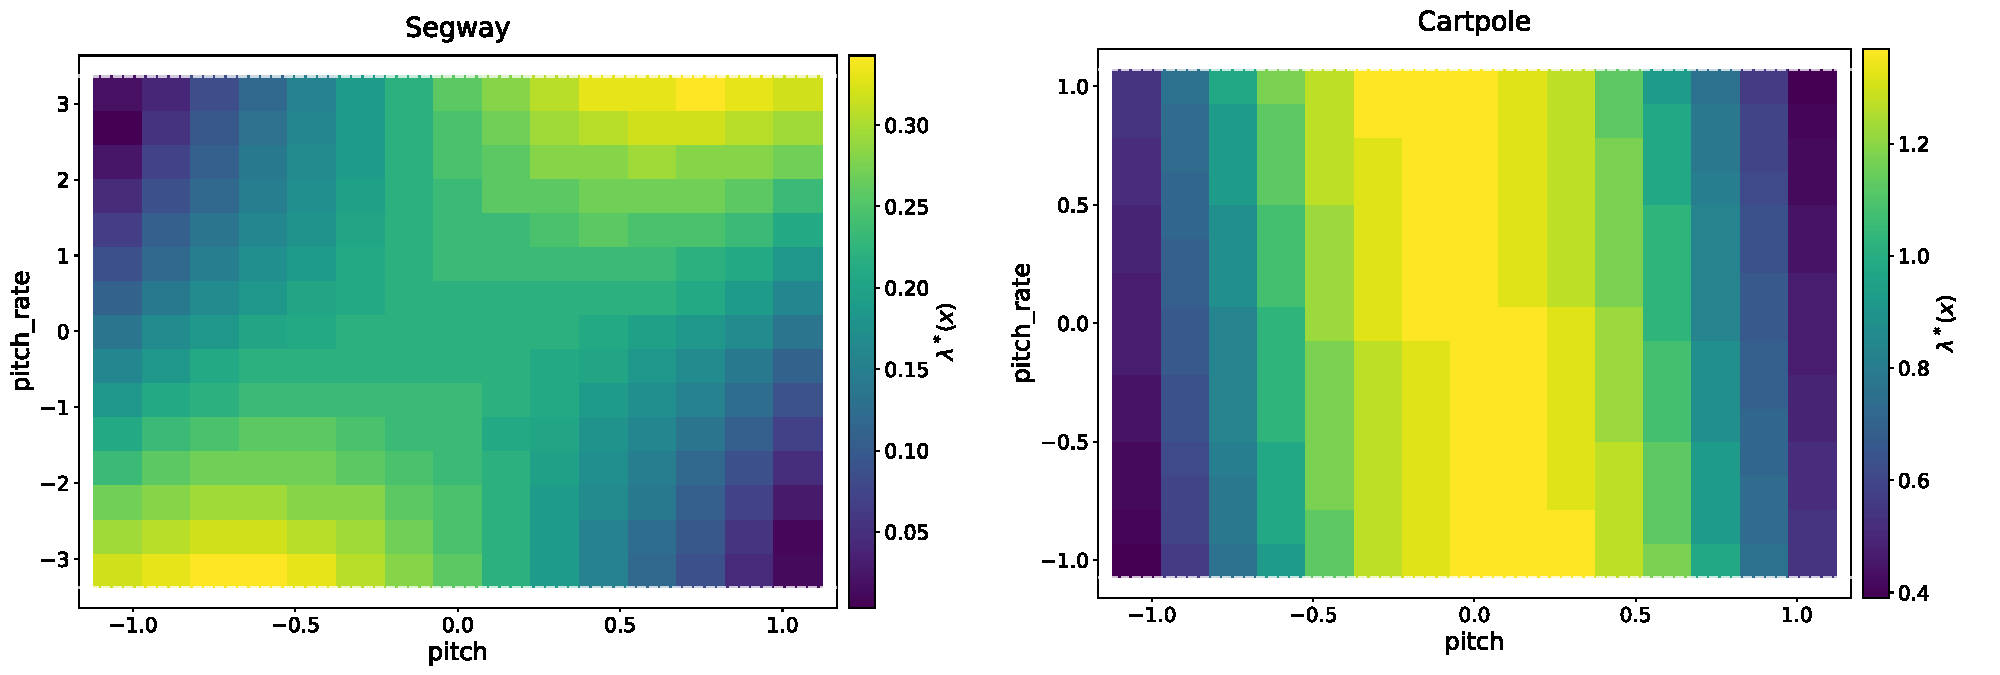
\includegraphics[width=0.99\linewidth]{fig/Presentation1.pdf}
    \caption{Certified rate $\lambda^*(x)$ over the each state subsets (grids). 
    The CartPole and Segway systems exhibit varying control authority ($\operatorname{tr}(BB^\top)$), confirming state-dependent optimal rates that vary by states. }
    \label{fig:placeholder}
\end{figure}



\section{State-Dependent IES for Optimal Policies}
We analyze the incremental exponential stability (IES) of the RL-trained optimal policy defined in \Cref{eqn:discounted_optimal_policy}, which accounts for the transient overshoot caused by prioritizing long-term optimality and state-dependent contraction rate.




We formally analyze the stability of the optimal policy defined in \Cref{eqn:discounted_optimal_policy} by establishing its state-dependent IES.
Let $\|\delta x(t)\|_M^2 \coloneq \delta x^\top M(x) \delta x$ represent the Riemannian energy defined by CCMs along the geodesic joining $x(t)$ and $x^*(t)$.
We define a reward function as follows:
\begin{equation}\label{eqn:reward_function}
    R(x, \delta x) = - \| \delta x\|_M^2,
\end{equation}
such that the optimal policy minimizes discounted cumulative Riemannian energy defined by CCMs.
While \cite{11664333} used normalized form of \Cref{eqn:reward_function} for numerical stability, we chose \Cref{eqn:reward_function} for analytical convenience. 

Throughout the analysis, we assume the existence of a set of contracting policies.
\begin{assumption}\label{assumption:1}
    Let $ \{ \mc{X}_n \}_{n=1}^{N}$ be a collection of nested, decreasing state subsets such that $\mc{X}_{n+1} \subset \mc{X}_n \subset \mc{X}_1 \coloneq \mc{X}$. For each $n = 1, 2, \dots, N$, there exists a deterministic contracting policy $\hat{\pi}_n$ that satisfies \Cref{eqn:contraction_condition} with respect to $\| \delta x(t) \|_M^2$ at a rate $\lambda_n$ as follows:
    \begin{equation}\label{eqn:contraction_inequality_star}
        \|\delta x(t_k)\|_M^2 \le \|\delta x(t_0)\|_M^2 e^{-2 \lambda_n k \Delta t},
        \; \forall k\in\mathbb N, \; \forall \delta x(t_0) \in \mc{X}_n,
    \end{equation}
    where $0< \lambda_1 < \lambda_2 < \dots < \lambda_N < \infty$, and each $\mc{X}_n$ is forward invariant under its respective contracting policy $\hat{\pi}_n$.
\end{assumption}

We depict a notional diagram of \Cref{assumption:1} in \Cref{fig:notional_diagram}a.



\subsubsection{State-Dependent IES}
Let $\pi^\star$ denote the optimizer of \Cref{eqn:discounted_optimal_policy} with the reward function defined in \Cref{eqn:reward_function}.
Let $\mc{S}_n \coloneq \mc{X}_n \times \mc{X}_n \times \mc{U}$ be augmented RL state space for state space $\mc{X}_n$.
We additionally define the state-dependent functions $\beta(s)$ and $\Lambda(s)$ used in the analysis as follows:
\begin{equation}\label{eqn:Lambda_function}
    \Lambda(s) \coloneqq 
    \begin{cases}
        \lambda_N, & \text{if } s \in \mc{S}_N, \\
        \lambda_n, & \text{if } s \in \mc{S}_n \setminus \mc{S}_{n+1},
    \end{cases}
\end{equation}

\begin{equation}\label{eqn:beta_function}
    \beta(s) \coloneqq 
    \begin{cases}
        (1-\gamma e^{-2 \lambda_N \Delta t})^{-1}, & \text{if } s \in \mc{S}_N, \\
        (1-\gamma e^{-2 \lambda_n \Delta t})^{-1}, & \text{if } s \in \mc{S}_n \setminus \mc{S}_{n+1},
    \end{cases}
\end{equation}
for $n = 1, 2, \dots, N-1$.

    

\begin{theorem}[State-Dependent IES]\label{theorem:acc_exp_stability_C}
    Suppose there exists a set of contracting policies $\{ \hat \pi_n\}_{n}^N$ as in \Cref{assumption:1}.
    Then, the optimal policy $\pi^\star$ of \Cref{eqn:discounted_optimal_policy} is incrementally exponentially stable at a state-dependent rate as follows:
    \begin{equation}\label{eqn:sd_IES}
       C(s_{k}) \leq \beta(s_0) C(s_0) e^{- 2 \overline{\lambda}(0, k) k \Delta t}, \quad \forall k \in \mb{N}, \; s_0 \in \mc{S},
    \end{equation}
    where $\beta(s)$ is defined in \Cref{eqn:beta_function}, $\overline{\lambda}(0, k) \coloneq k^{-1} \sum_{k'=0}^{k-1} \Lambda(s_{k'})$, and $\Lambda(s)$ is defined in \Cref{eqn:Lambda_function}.
\end{theorem}
\begin{proof}
    See Appendix \ref{app:proof_theorem1}.
\end{proof}

\Cref{fig:notional_diagram}b illustrates a notional state-dependent contraction bound, which permits the potentially faster contraction rates established in \Cref{theorem:acc_exp_stability_C}.




\begin{corollary}[Nominal IES]\label{rem:nominal_recovery}
When \Cref{assumption:1} is restricted to a single subset ($N = 1$), \Cref{theorem:acc_exp_stability_C} reduces to the nominal IES at the uniform rate $\lambda_1$. 
Furthermore, restricting $\gamma \rightarrow 0$ gives overshoot-free nominal contracting policy.
\end{corollary}



\begin{remark}[Advantages of Minimizing Error Defined by Contraction Metrics]\label{remark:advantages_of_Riemannian_energy}
    An optimal policy that minimizes the Euclidean error (i.e., $\| \delta x \|_I^2$) does not guarantee IES under the framework of \Cref{theorem:acc_exp_stability_C}, unless the dynamics in \Cref{eqn:control_affine_system} admit $I$ as contraction metrics.
\end{remark}
\begin{proof}
    See Appendix \ref{app:proof_of_remark}.
\end{proof}

% \begin{remark}[Comparison to traditional IES]\label{remark:2}
%     Given \Cref{theorem:acc_exp_stability_C}, taking the limit as $\gamma \to 0^+$ enables the synthesis of an overshoot-free contracting policy that achieves an accelerated contraction rate within the Riemannian space defined by CCMs.
% \end{remark}
% \Cref{remark:2} provides a distinct advantage over prior approaches to the synthesis of contracting policies, which merely guarantee overshoot-free nominal contraction.

\begin{remark}[Comparison to IES Established in \cite{11664333}]
    \cite{11664333} does not account for transient overshoot when proving the IES of the optimal policy $\pi^\star$, resulting in a conservative guarantee where IES holds only if the discount factor is below a certain threshold. 
    In contrast, \Cref{theorem:acc_exp_stability_C} holds for any discount factor $\gamma \in (0, 1)$ by accounting for the transient overshoot introduced by long-term optimality via $\beta(s_0)$.
    % Additionally, \Cref{theorem:acc_exp_stability_C} shows the optimal policy can leverage accelerated contraction once dynamics permit it.
\end{remark}




% \begin{figure}
%     \centering
%     \includegraphics[width=0.95\linewidth]{figs/algorithm.pdf}
%     \caption{The workflow depicts the schematic of interdependencies between CCM generater, policies with $\gamma \rightarrow 0$ and $\gamma \rightarrow 1$ during training. 
%     During policy optimization, the generated CCMs are used to define the Riemannian energy that the policy minimizes.}
%     \label{fig:algorithm}
% \end{figure}



% \section{Algorithm}
% We propose an RL algorithm to empirically validate the theoretical guarantees established in \Cref{theorem:acc_exp_stability_C}.

% \subsubsection{Markov decision process for nonlinear control}
% Following \cite{11664333}, we formulate the nonlinear control problem as a Markov decision process (MDP) $\mc{M} \coloneq (\mc{S}, \mc{U}, R, T)$.
% The state space is defined as $\mc{S}\coloneq (x, \vec{x}^*, u^*)$, where $x$ is the current state, $\vec{x}^*$ is the sequence of reference states, and $u^*$ is the reference control.
% The control space is denoted by $\mc{U}$, and we generate the control at each time step $t$ using the following parameterization:
% \begin{equation}
%     u_t = u^*_t + \Theta_1(\vec{x}^*) \tanh\big(\Theta_2(x_t) (x_t - x^*_t)\big),
% \end{equation}
% where $\Theta_1: \mb{R}^{n \cdot H} \rightarrow \mb{R}^{m \times h}$ is parameterized by a recurrent neural network, and $\Theta_2: \mb{R}^n \rightarrow \mb{R}^{h \times n}$ is a standard neural network. 
% Here, $H = (1-\gamma)^{-1}$ represents the effective horizon, and $h$ is the latent feature dimension.

% Because exact geodesic computation is computationally intractable, we approximate the tracking reward defined in \Cref{eqn:reward_function} using a local Riemannian energy metric based on Euclidean displacement. Furthermore, to ensure numerical stability during training, we frame this approximation using potential-based reward shaping \cite{ng1999policy}:
% \begin{equation}\label{eqn:practical_reward_function}
%     R(s_t) = -\| \delta \hat{x}_{t+1}\|_M^2 + \| \delta \hat{x}_{t}\|_M^2,
% \end{equation}
% where $\| \delta \hat{x}_t\|_M^2 \coloneq (x_t - x^*_t)^\top M(x_t) (x_t - x^*_t)$.
% This potential-based reward shaping improves sample efficiency by driving policy updates based on the stepwise reduction in tracking error, rather than being overwhelmed by the absolute magnitude of the error. Furthermore, it strictly preserves the optimal policy, with the formal proof provided in Appendix \ref{app:path_tracking_reward}.
% The transition dynamics $T: \mc{S} \times \mc{U} \rightarrow \mc{S}$ are deterministic.

% \subsubsection{Architecture}
% Our proposed algorithm---certified control using reinforcement learning (C2RL)---consists of a three-stage process for each environment: (a) computing a uniform contraction rate and its corresponding contraction metrics, (b) training a neural contraction metric, and (c) optimizing the control policy.
% We depict the overall algorithm in \Cref{fig:algorithm}.

% Stages (a) and (b) follow the methodology introduced in \cite{tsukamoto2020robust, tsukamoto2020neural}. Specifically, we apply the ConVex optimization-based Steady-state Tracking Error Minimization (CV-STEM) method to identify the highest uniform contraction rate across the state set $\mc{X}$ by solving the following optimization problems:
% \begin{align}
%     \min_{\bar{W}_k,\,\nu,\,\chi} \quad & c_0\chi + c_1\nu \\
%     \text{s.t.} \quad & I \preceq \bar{W}_k \preceq \chi I, \quad \forall k \in \{1,\dots,N\}, \\
%     & S_k \preceq -\varepsilon I, \quad \forall k \in \{1,\dots,N\}, \\
%     & \nu > 0, \quad \nu \leq \underline{w}^{-1}, \quad \chi \leq \nu \overline{w},
% \end{align}
% where $c_0$ penalizes the steady-state tracking error, $c_1$ penalizes the feedback gain, and $S_k$ is defined as 
% \begin{equation}
%     S_k = \dot{\bar{W}}_k + A_k \bar{W}_k + \bar{W}_k A_k^\top + 2\lambda \bar{W}_k - \nu\left(\frac{2}{r}\right)B_k B_k^\top.
% \end{equation}
% Finally, $\varepsilon \geq 0$ allows for the extension of pointwise contraction to continuous time, given sufficient smoothness.

% We chose $c_0 = 1/\lambda$ and $c_1 = 1$ to recover the reference objective $\bar{d}_c\chi/\alpha + d_2\nu$ under a unit disturbance bound $\bar{d}_c = 1$ and unit gain penalty $d_2 = 1$, the $1/\lambda$ being the $1/\alpha$ that the error bound places there rather than a free hyperparameter.

% Then, the deployed metric is recovered by undoing the normalisation $\bar{W} = \nu W$:
% \begin{equation}
%     M(x_k) = W(x_k)^{-1} = \left(\frac{\bar{W}_k}{\nu}\right)^{-1} = \nu\,\bar{W}_k^{-1}.
% \end{equation}

% We then train a deep neural network parameterized by $\Phi:\mb{R}^n \rightarrow \mb{R}^{n \times n}$ to regress these contraction metrics by minimizing the following loss:
% \begin{equation}
%     \Phi^\star = \arg\min_{\Phi} \frac{1}{N} \sum_{k=1}^N \big\| M_\Phi(x_k) - M(x_k) \big\|_F^2.
% \end{equation}

% Here, we structurally ensure that the generated metric stays inside the deployment envelope (i.e., $\underline{w}I \preceq W_\Phi = M_\Phi^{-1} \preceq \overline{w}I$) by using the eigendecomposition of the positive definite contraction metric $M(x) = V\Lambda V^{\!\top}$:
% \begin{equation}
%     M_\Phi(x) = V \operatorname{diag}\!\Big( \underline{w} + (\overline{w} - \underline{w}) \sigma(\lambda_i) \Big) V^{\!\top},
% \end{equation}
% where $\lambda_i$ are the eigenvalues and $\sigma(\cdot)$ is the sigmoid function.

% Stage (c) performs policy optimization to maximize the discounted sum of rewards, as formulated in \Cref{eqn:practical_reward_function}, where the state-dependent metric $M$ is dynamically generated by the trained neural network as follows:
% \begin{equation}
%     \pi^\star = \argmax_{\Theta_1, \Theta_2} 
% \end{equation}
% where we use GRU for $\Theta_1$ to encode a long sequence of reference trajectories and ..



% \section{Experiments}\label{sec:experiments}
% In this section, we perform empirical study to complement \Cref{theorem:acc_exp_stability_C} and \Cref{remark:advantages_of_Riemannian_energy} by answering the following questions:
% \begin{enumerate}
%     \item Does the optimal policy trained with high discount factor exchange transient overshoot with future accelerated contraction?
%     \item How does the optimal policy compare to an optimal policy minimizing Euclidean error.
%     \item Does the optimal policy trained with $\gamma \rightarrow 0$ outperforms contracting policies synthesized by prior approaches?
%     % \item Can the optimal policy achieve accelerated contraction at the expense of overshoot in both linear (with a perfect contraction metric) and nonlinear (with an imperfect contraction metric) dynamics?
%     % \item How does the discount factor affect the duration of accelerated contraction and the resulting overshoot?
%     % \item Can we relate contraction violations to the metric approximation error $\eta$?
%     % \item Can the proposed algorithm perform better than naive approaches?
% \end{enumerate}

% We answer these questions across a diverse range of environments including traditional mobile robots (TurtleBot, Car, PVTOL, and Quadrotor), where we exactly formulate CCM conditions, and high-dimensional complex dynamical systems (Manipulator, Quadruped, and Humanoid), we approximate the CCM conditions using a data-driven approach. 
% Details regarding these environments are provided in Appendix \ref{app:env_details}.


% \subsection{Horizon Setting}
% We set N horizon and set contraction metric bound such that it decays at least $95\%$ of initial error for $\lambda = 0.5$ for 15 seconds.


% \subsection{When overshoot happens?}


\section{Toy Problems}\label{sec:toy}
In this section, we use two nonlinear polynomial dynamical systems, 
for which exact contraction metrics and our proposed optimal controls can be derived, 
to illustrate \Cref{theorem:acc_exp_stability_C} by answering the following questions:
\begin{enumerate}
    \item Does the optimal control policy satisfy the state-dependent contraction bounds established in \Cref{theorem:acc_exp_stability_C}?
    \item Does the discount factor systematically correlate with the running mean contraction rate, overshoot, and cumulative error?
\end{enumerate}

To answer these questions, we use a $\lambda$-ascent reference control, which we describe in \Cref{subsubsec:lambda_ascent}, to generate a reference trajectory
from an arbitrary initial condition to satisfy the forward-invariance contraction rate in \Cref{assumption:1}.
For comparison, we generate another reference trajectory from the same initial condition 
using a stabilizing control, which we describe in \Cref{subsubsec:stabilizing_ref}, to illustrate the system's behavior when the forward invariance does not hold.



\subsection{Polynomial Dynamical Systems}
We consider the two-dimensional state and one-dimensional control ($n=2, m=1$) 
Moore--Greitzer jet-engine model \cite{moore1986theory} and the Duffing double-well oscillator \cite{guckenheimer1983nonlinear} 
and show their control-affine dynamics in \Cref{eqn:toy_mg} and \Cref{eqn:toy_duff}, respectively.

\subsubsection{Control-Affine Forms}
\textbf{Moore--Greitzer jet-engine model.}
The Galerkin-projected post-stall compressor model is given by:
\begin{equation}\label{eqn:toy_mg}
    \begin{aligned}
        \dot{x}_1 &= -x_2 - \tfrac{3}{2}x_1^2 - \tfrac{1}{2}x_1^3, \\
        \dot{x}_2 &= 3x_1 + u,
    \end{aligned}
\end{equation}
where $x_1$ is the mass flow, $x_2$ is the pressure rise, 
and the control input $u$ represents the throttle setting.
The control problem here is to stabilize the system at the origin, 
which is a non-hyperbolic equilibrium of the open-loop dynamics, 
so the drift alone does not stabilize it.

\textbf{Duffing double-well oscillator.}
The normalized Duffing oscillator, with stiffness $\alpha = 1$, softening coefficient $\beta = \tfrac{1}{3}$, 
and damping $\delta = \tfrac{3}{10}$, is given by:
\begin{equation}\label{eqn:toy_duff}
    \begin{aligned}
        \dot{x}_1 &= x_2, \\
        \dot{x}_2 &= -x_1 + \tfrac{1}{3}x_1^3 - \tfrac{3}{10} x_2 + u,
    \end{aligned}
\end{equation}
where $x_1$ is the position, $x_2$ is the velocity, 
and the control input $u$ represents the external force applied to the oscillator. 
The control problem here is again to stabilize the system at the origin, 
which is a stable focus of the open-loop dynamics but only locally: 
the cubic term places saddle equilibria at $(\pm\sqrt{3}, 0)$ inside the state space, 
so the drift alone does not stabilize it either.

\subsubsection{MDP Setting}
Each of systems above will be simulated in discrete time $dt = 0.05$ and $H=100$ timesteps, 
so $T = H \Delta t = 5$\,s. 
The state space is $\mathcal{X} = [-1.5, 1.5] \times [-2.5, 2.5]$ for \eqref{eqn:toy_mg} 
and $\mathcal{X} = [-2.5, 2.5]^2$ for \eqref{eqn:toy_duff}, 
and the control space is $\mathcal{U} = [-6, 6]$ and $\mathcal{U} = [-8, 8]$, respectively, 
each twice the box from which the reference control is drawn so that feedback always has authority to spare. 
The rationale behind these numbers is to choose a fine enough discretization to reduce the numerical integration error, 
and also to ensure the given tracking admits a $95\%$ reduction of the initial Riemannian energy over the horizon. 
The latter holds because $T$ exceeds $1.5 / \min_x \lambda(x)$ on both domains, 
which is $3.06$\,s for \eqref{eqn:toy_mg} and $1.45$\,s for \eqref{eqn:toy_duff}. 
We hold $H$ fixed across every discount factor, 
so that the execution length remains a property of the task rather than of $\gamma$.

\subsubsection{Existence of State-Dependent Contraction Rates}
Both plants share the constant input matrix $B = [\,0 \;\; 1\,]^\top$, 
so $\operatorname{tr}(BB^\top)$ is constant and \Cref{prop:orthogonal_test} is decided by the drift Jacobian $A(x) = \partial f / \partial x$ alone. 
Applying the same trace test to $A$, the Moore--Greitzer model \eqref{eqn:toy_mg} gives 
$\operatorname{tr}(A(x)A(x)^\top) = (3x_1 + \tfrac{3}{2}x_1^2)^2 + 10$, 
which ranges from $10.000$ to $72.016$ over $\mathcal{X}$, 
while the Duffing oscillator \eqref{eqn:toy_duff} gives 
$\operatorname{tr}(A(x)A(x)^\top) = (x_1^2 - 1)^2 + 1.09$, ranging from $1.090$ to $28.652$. 
Because this invariant scalar fluctuates in both systems, no orthogonal reduction $T(x)$ can exist, 
which confirms that both plants admit state-dependent contraction rates. 
The certified rate fields of \Cref{app:proof_toy_problems} realize this, 
varying by $4.98\times$ for \eqref{eqn:toy_mg} and $1.84\times$ for \eqref{eqn:toy_duff}.

\subsubsection{Stabilizing Reference Control}\label{subsubsec:stabilizing_ref}
Since neither drift is stabilizing over its domain, the reference trajectory of \eqref{eqn:ref_rollout} cannot be generated with $u^* = 0$. 
For the Moore--Greitzer model, we apply the stabilizing control law $u^*(x) = -x_2$ to generate a reference trajectory for an arbitrary (unstable) initial condition, 
while for the Duffing oscillator, we utilize $u^*(x) = -2x_1$, 
which is the cancellation $u = -(\alpha + k_1)x_1$ with $k_1 = 1$ and needs no derivative term because the plant already carries the damping $\delta$. 
Both closed loops are Hurwitz at the origin, with eigenvalues $-0.5 \pm 1.658\jmath$ and $-0.15 \pm 1.726\jmath$ respectively, 
and are certified asymptotically stable over the entire $\mathcal{X}$ by a quartic Lyapunov function, 
while no quadratic certificate exists for either. 
We detail this in \Cref{app:proof_toy_problems}.

\subsubsection{$\lambda$-Ascent Reference Control}\label{subsubsec:lambda_ascent}
The stabilizing reference stays where it starts in the rate field, so it never exercises the ordering of \Cref{assumption:1}. 
To exercise it, we instead choose $u^*$ to climb the rate field, 
differentiating $\lambda$ along \eqref{eqn:ref_rollout} and selecting the admissible input that maximizes $\dot{\lambda}$. 
The reference then begins in a low-rate region and migrates to a high-rate one while remaining a trajectory of the plant. 
We describe the law and the states at which a rate can actually be held in \Cref{app:ascending_ref}.


\subsection{Contraction Metric Synthesis using SoS Programming}
We follow \cite{aylward2008stability} that imposes the contraction condition as an algebraic identity rather than at sampled states. 
A polynomial $p$ is nonnegative on the box $\mathcal{X} = \prod_i [\underline{x}_i, \overline{x}_i]$ 
whenever it admits the representation $p = \sigma_0 + \sum_i \sigma_i b_i$ 
with every $\sigma_j$ a sum of squares (SoS) and $b_i(x) \coloneq (x_i - \underline{x}_i)(\overline{x}_i - x_i)$ \cite{putinar1993positive}, 
and this representation is itself found by semidefinite programming \cite{parrilo2000structured}. 
Writing the matrix inequality \eqref{eqn:app_S} as a scalar polynomial in an auxiliary variable $v \in \mathbb{R}^n$ 
and certifying each resulting polynomial in this form, we solve the following optimization:
\begin{equation}\label{eqn:toy_sos}
    \begin{aligned}
        \max_{\lambda, \, W, \, \{\sigma_j\}} \quad & \lambda \\
        \text{s.t.} \quad
        & -v^\top S(x) v = \sigma_0 + \textstyle\sum_i \sigma_i b_i, \\
        & \;\;\; v^\top (W(x) - \underline{w} I) v = \sigma'_0 + \textstyle\sum_i \sigma'_i b_i, \\
        & \;\;\; v^\top (\overline{w} I - W(x)) v = \sigma''_0 + \textstyle\sum_i \sigma''_i b_i, \\
        & \sigma_j, \, \sigma'_j, \, \sigma''_j \ \text{SoS},
    \end{aligned}
\end{equation}
where $S \coloneq \dot{W} + AW + WA^\top + 2\lambda W - \tfrac{2}{r}BB^\top$ stands for the CV-STEM operator of \eqref{eqn:app_S} 
with $A \coloneq \partial f / \partial x$ and $\dot{W} = \sum_i (\partial W / \partial x_i) f_i$, 
and $\underline{w}, \overline{w}$ stand for the bounds on the spectrum of the dual metric $W = M^{-1}$. 
We take each entry of $W$ of total degree $2$, with $\underline{w} = 0.1$, $\overline{w} = 10$, and $r = 0.1$. 
Since $\lambda$ multiplies $W$, the program is bilinear and we solve it by bisection on $\lambda$, 
each trial being a single linear SDP.

Intuitively, the output contraction metric is analytical expressions in terms of state $x$
whose condition number over $\mathcal{X}$ is bounded by $27.7$ for \eqref{eqn:toy_mg} and $34.0$ for \eqref{eqn:toy_duff},
and is exact under the criterion that the certified inequality holds at every point of $\mathcal{X}$ rather than at a finite draw from it.
Note that this differs from contraction metric synthesis approach CV-STEM \eqref{eqn:cvstem1}--\eqref{eqn:cvstem4}, 
which we will use for non-polynomial nonlinear systems in \Cref{sec:state_dependent_examples},
and the reason is CV-STEM is sample-based and does not provide analytical expressions of contraction metrics
but in sample wise to reduce any approximation and estimation errors.
The certified condition is identical in both, so the rates the two families report remain directly comparable, 
and we compare them in \Cref{app:sos_vs_cvstem}.


\subsection{Optimal Control Synthesis using SoS Programming}
Given the certified metric, the benchmark optimal control is the global minimizer 
of the discounted tracking cost over the same discrete-time plant:
\begin{equation}\label{eqn:toy_pop}
    \begin{aligned}
        \min_{u_{0:H-1}} \quad & \textstyle\sum_{t=0}^{H-1} \gamma^t c(x_t, u_t) \\
        \text{s.t.} \quad & x_{t+1} = x_t + \Delta t \, (f(x_t) + B u_t), \\
        & x_t \in \mathcal{X}, \quad u_t \in \mathcal{U},
    \end{aligned}
\end{equation}
where $x_0$ is fixed and $c$ stands for the negated reward of \eqref{eqn:reward_function}, 
written in the potential-shaped form $c(x_t, u_t) = -q (V_t - V_{t+1}) + r \|u_t\|^2$ 
with $V_t \coloneq \|x_t - x^*_t\|_{M(x_t)}^2$. 
This is a nonconvex polynomial optimization problem, 
for which the moment-SoS hierarchy \cite{lasserre2001global} produces a monotone sequence of certified lower bounds.

A dense hierarchy is not viable here, since the number of nonconvex variables is $3H$ and therefore grows with the horizon; 
a discount sweep would then return certified optima at low $\gamma$ and timeouts at high $\gamma$. 
We instead exploit the chain structure of \eqref{eqn:toy_pop}, in which $x_{t+1}$ couples only to $(x_t, u_t)$, 
through correlative sparsity \cite{waki2006sums, lasserre2006convergent}. 
This decomposes the relaxation into cliques whose size is independent of $H$, 
so that the cost grows linearly in the horizon.

Two reformulations expose that structure. 
First, the decrement cost telescopes into a positive weighted sum of the levels $V_t$, 
which removes the cross terms and places every objective monomial on a single clique. 
Second, the certificate is written in $W$, so $M = W^{-1}$ is rational; 
we lift each level to an epigraph variable $v_t$ constrained by 
$v_t \det W(x_t) \ge (x_t - x^*_t)^\top \operatorname{adj} W(x_t) (x_t - x^*_t)$, 
which is polynomial and tight at the optimum since $\det W > 0$ on $\mathcal{X}$ and the weights are positive. 
The resulting cliques are $\{x_t, u_t, x_{t+1}\}$ and $\{x_t, v_t\}$, 
ordered so that the running-intersection property holds, 
and we relax them at orders $3$ and $4$ respectively.

The relaxation returns a certified lower bound on \eqref{eqn:toy_pop}, 
while its first-order moments return a candidate input sequence 
whose rollout through the environment gives a feasible upper bound. 
The two bracket the global optimum, so every optimal control reported below 
carries a certificate of how far it can be from optimal.



HOW TO ANSWER EACH QUESTIONS


\section{Conclusion}
In this paper, we proposed a theoretical condition to determine whether control-affine systems exhibit state-dependent contraction rates. Building on this, we established state-dependent contraction bounds for optimal policies trained via reinforcement learning (RL) to minimize cumulative tracking errors. Crucially, we demonstrated that through RL policy optimization, these bounds decay at the highest feasible contraction rate for any given state, even when the underlying contraction metric relies on a conservative, uniform rate. Future work will focus on rigorous empirical validation of these theoretical guarantees, specifically verifying that accelerated error decay is actively realized in regions of the state space that admit higher contraction rates.

% \section*{Acknowledgments}
% This should be a simple paragraph before the References to thank those individuals and institutions who have supported your work on this article.



\appendices
% cleveref numbers appendices as sections; alias them so \Cref prints
% "Appendix" rather than "Section".
\crefalias{section}{appendix}
\crefalias{subsection}{appendix}

\section{Proof of \Cref{theorem:acc_exp_stability_C}}\label{app:proof_theorem1}

We introduce the following two lemmas to prove \Cref{theorem:acc_exp_stability_C}.
\begin{lemma}[Sandwiched Value Function]\label{lemma:value_sandwich}
    % Suppose there exists contracting policies $\pi_c$ within $\mc{X}$ as in \Cref{assumption:1} and $\pi_{c^*}$ within $\mc{X}^*$ as in \Cref{assumption:2}.
    Suppose there exists a set of contracting policies $\{ \hat \pi_n\}_{n}^N$ as in \Cref{assumption:1}.
    Then, the cost value function for the optimal policy $\pi^\star$ of \Cref{eqn:discounted_optimal_policy} satisfies the following inequality:
    \begin{equation}
        C(s) \leq V^{\pi^\star}_{C}(s) \leq \beta(s) C(s), 
    \end{equation}
    where $\beta(s)$ is defined in \Cref{eqn:beta_function}.
\end{lemma}
\begin{proof}
    The lower bound holds trivially for $C \ge 0$, as the value function is the sum of non-negative costs.
    The upper bound follows from the optimality of $\pi^\star$, yielding
    \begin{align}
        V^{\pi^\star}_C(s) & \leq V^{\pi_{c^*}}_C(s) \leq \frac{C(s)}{1 - \gamma e^{-2 \lambda_N \Delta t}}, \quad \forall s \in \mc{S}_N, \\ 
        V^{\pi^\star}_C(s) & \leq V^{\pi_c}_C(s) \leq \frac{C(s)}{1 - \gamma e^{-2 \lambda_n \Delta t}}, \quad \forall s \in \mc{S}_n \setminus \mc{S}_{n+1},
    \end{align}
    where we use the convergence of a geometric series.
\end{proof}

\begin{lemma}[Value Contraction]\label{lemma:value_contraction}
    % Suppose there exists contracting policies $\pi_c$ within $\mc{X}$ as in \Cref{assumption:1} and $\pi_{c^*}$ within $\mc{X}^*$ as in \Cref{assumption:2}.
    Suppose there exists a set of contracting policies $\{ \hat \pi_n\}_{n}^N$ as in \Cref{assumption:1}.
    Let $\Lambda(s)$ be defined as in \Cref{eqn:Lambda_function}.
    Then, the cost value function for the optimal policy $\pi^\star$ of \Cref{eqn:discounted_optimal_policy} achieves contraction at a running mean rate as follows:
    \begin{equation}\label{eqn:value_contraction_C}
        V^{\pi^\star}_{C}(s_{k}) \leq V^{\pi^\star}_{C}(s_0) e^{-2 \overline{\lambda}(0, k) k \Delta t}  , \quad \forall k \in \mb{N}, \; s_0 \in \mc{S},
    \end{equation}
    where $\overline{\lambda}(0, k) \coloneq k^{-1} \sum_{k'=0}^{k-1} \Lambda(s_{k'})$ is the running average contraction rate along the trajectory.
\end{lemma}
\begin{proof}
    Suppose the cost $C$ is nonzero, so is $V_C^{\pi^\star}$. 
    Given the deterministic dynamics and the deterministic optimal policy, we begin with the Bellman optimality equation:
    \begin{equation}
        V^{\pi^\star}_C(s_t) = C(s_t) + \gamma V^{\pi^\star}_C(s_{t+1}),
    \end{equation}
    which can be rearranged to isolate the contraction factor:
    \begin{equation}
        V^{\pi^\star}_C(s_{t+1}) = \underbrace{ \gamma^{-1}\left( 1 - \frac{C(s_t)}{V^{\pi^\star}_C(s_{t})} \right)}_{\rho(s_t)}V^{\pi^\star}_C(s_{t}).
    \end{equation}
    Dividing the upper bounds in \Cref{lemma:value_sandwich} by $V^{\pi^\star}_C(s_t) > 0$ yields:
    \begin{equation}\label{eqn:beta_prime_value_bound}
        1 \leq \beta(s_t) \frac{C(s_t)}{V^{\pi^\star}_C(s_t)} \implies {\beta(s_t)}^{-1} \le \frac{C(s_t)}{V^{\pi^\star}_{C}(s_t)} \leq 1, \; \forall s_t \in \mc{S}.
    \end{equation}
    Rearranging \Cref{eqn:beta_prime_value_bound} and scaling by $\gamma^{-1}$ establishes the following uniform bounds on $\rho(s_t)$:
    \begin{equation}
        \rho(s_t) \leq \gamma^{-1}\big(1-{\beta(s_t)}^{-1}\big) = e^{-2 \Lambda(s_t) \Delta t} < 1, \quad \forall s_t \in \mc{S},
    \end{equation}
    which yields the step-wise value contraction:
    \begin{equation}
        V^{\pi^\star}_C(s_{t+1}) \leq e^{-2 \Lambda(s_t) \Delta t} V^{\pi^\star}_C(s_{t}).
    \end{equation}
    Recursively applying the value contraction over $k$ steps gives:
    \begin{align}
        V^{\pi^\star}_C(s_{t+k}) & \leq V^{\pi^\star}_C(s_{t}) \prod_{k'=0}^{k-1} e^{-2 \Lambda(s_{t + k'}) \Delta t} \\
        &= V^{\pi^\star}_C(s_{t}) e^{-2 \overline{\lambda}(t, t+k) k \Delta t},
    \end{align}
    where $\overline{\lambda}(t, t+k) \coloneq k^{-1} \sum_{k'=0}^{k-1} \Lambda(s_{t+k'})$ denotes the running average contraction rate along the trajectory. 
    % Setting $t = 0$ gives \Cref{eqn:value_contraction_C}.
\end{proof}



\begin{proof}[\textbf{Proof of \Cref{theorem:acc_exp_stability_C}}]
    Applying the value sandwich inequality (see \Cref{lemma:value_sandwich}) to the value contraction inequality (see \Cref{lemma:value_contraction} gives the desired results as follows:
    \begin{align}
        V^{\pi^\star}_{C}(s_{t + k}) & \leq  V^{\pi^\star}_{C}(s_t) e^{- 2 \overline{\lambda}(t, t+k) k \Delta t} \\
        \implies & C(s_{t + k}) \leq \beta(s_t) C(s_t) e^{- 2 \overline{\lambda}(t, t+k) k \Delta t},
    \end{align}
    for all $ k \in \mb{N}$ and $ s_t \in \mc{S}$. Setting $t = 0$ gives \Cref{eqn:sd_IES}.
\end{proof}




\section{Proof of \Cref{remark:advantages_of_Riemannian_energy}}\label{app:proof_of_remark}

The optimal policy minimizing Euclidean error satisfies \Cref{lemma:value_sandwich} with an additional slack term, $\sqrt{\overline{m}/\underline{m}}$, as the contraction bound of policy $\hat \pi_n$ in Euclidean space becomes:
\begin{equation}
    C(s_{k}) \leq \sqrt{\overline{m}/\underline{m}} C(s_0) e^{- \lambda k \Delta t}, \quad \forall k \in \mb{N}, \; s_0 \in \mc{S}.
\end{equation}
This renders \Cref{eqn:beta_prime_value_bound} invalid; consequently, the value contraction in \Cref{lemma:value_contraction} is no longer guaranteed.


\section{Computation of the Contraction-Rate Field}\label{app:rate_field}

We detail the procedure summarized in \Cref{sec:state_dependent_examples} and
the conditions under which it is valid. Throughout, $\mathcal{Q}$ denotes the
finite set of query states at which the field is evaluated.

\paragraph{Two Estimators}
The map $x\mapsto\lambda^*(x)$ of \eqref{eq:lambda_star_x} admits two distinct
finite-sample surrogates, and they answer different questions:
\begin{itemize}
    \item \emph{Certified.} Solve \eqref{eqn:cvstem1}--\eqref{eqn:cvstem4}
    \emph{once} over all of $\mathcal{Q}$ at the prescribed uniform rate, then
    report the local rate of the resulting single metric field at each query
    state,
    \begin{equation}\label{eqn:local_rate}
        \lambda(x) \coloneq
        -\tfrac{1}{2}\,\lambda_{\max}\!\bigl(\widehat{M A_{\mathrm{cl}}},\,M\bigr),
        \quad A_{\mathrm{cl}} \coloneq A - \tfrac{1}{r}BB^\top M,
    \end{equation}
    where $\lambda_{\max}(\cdot,\cdot)$ denotes the largest generalized
    eigenvalue and the arguments are omitted for brevity.
    This is the rate of the metric that is actually deployed.
    \item \emph{Ceiling.} Re-solve the program independently at each query state
    and report $\lambda^*(\{x\})$ by search over $\lambda$. This is the rate
    attainable if the metric were redesigned for that state alone; it upper
    bounds the certified rate and is not realized by any single controller.
\end{itemize}
Both are invariant under the orthogonal congruence of
\Cref{prop:orthogonal_test}, hence exactly constant on uniform-rate plants.
\Cref{fig:placeholder} reports the certified estimator. If the joint program is
infeasible at the prescribed rate, this is a statement about the certified
envelope of the plant and not a failure of the visualization; it must be
reported as such rather than worked around by lowering $\lambda$.

\paragraph{Marginalization}
Two of the $n$ dimensions are gridded and the remainder are marginalized by
minimization, which is the worst-case certification required for a bounded
subset: reporting an average or a single slice would claim a rate that does not
hold on part of the cell. Only \emph{active} dimensions---those on which
$A(\cdot)$ and $B(\cdot)$ actually depend---are sampled; inactive dimensions,
in particular the translation directions of $\mathcal{X}$, are pinned at the box
center. Randomizing an inactive dimension inflates the sample count without
adding a single distinct constraint, and any spread it appears to produce is
solver noise.

\paragraph{Actuator Feasibility}
A certificate is admissible only if the induced feedback respects
$\mathcal{U}$, so each cell is additionally screened on
\begin{equation}\label{eqn:viol_gate}
    \Pr\nolimits_{\delta x,u^*}\bigl[\,u^* - \tfrac{1}{r}B^\top M\,\delta x \notin \mathcal{U}\,\bigr] \le \eta,
    \qquad \eta = 0.05,
\end{equation}
estimated by Monte Carlo. The number of draws is not a free parameter. The gate
is evaluated one state at a time, so the draw count \emph{is} the entire sample:
at $64$ draws the estimator's standard deviation is $0.023$ against a budget of
$\eta=0.05$, and for a plant whose true violation rate sits $0.65\sigma$ below
the budget this rejects $25.7\%$ of cells at random---$17.3\%$ observed on the
car. Because a rejected cell falls back to a lower reported rate, the coin flip
is drawn directly into the figure as spatial structure. We use $2\times10^3$
draws per cell.

A residual ripple in \eqref{eqn:viol_gate} survives any draw count and is not
noise. Constructing $W(\psi)=T(\psi)W_0T(\psi)^\top$ from the exact symmetry of
\Cref{prop:orthogonal_test}---no solver in the loop, so the true rate is
constant by construction---still yields a violation rate ranging over
$0.02585$--$0.02704$, a peak-to-peak spread of $3.3\sigma$ at $2\times10^5$
draws. The cause is a frame mismatch: $\delta x$ is drawn from a fixed
box in world coordinates while $K(x)=r^{-1}B^\top M$ co-rotates with the state,
so the gate measures the box, not the plant. The draw box must be expressed in
the same frame as the gain.

\paragraph{Resolution}
Searching $\lambda$ on a fixed geometric ladder $\lambda\in[0.01,60]$ of $L$
points reports only ladder values, so the coarsest spread the estimator can
express is one bin, $(60/0.01)^{1/(L-1)}$. At $L=24$ this equals $1.4597$, and
every spread we initially measured was an integer power of it ($1.46$, $2.131$,
$3.110$, $20.613$), with as few as two distinct values across $225$ cells: the
reported state dependence was the ladder. Feasibility in $\lambda$ is
non-monotone---$\chi$ carries weight $c_0$, so the realizable set is an interval
rather than a ray---which is why the ladder is swept rather than bisected. We
therefore keep the sweep to bracket the interval and then bisect only between
the last feasible ladder point and its successor, to a relative tolerance of
$5\times10^{-3}$, at a cost of $24$--$40$ solves per cell.

\paragraph{Declaring a Field Constant}
Whether a field is constant is a scale-free question and must be tested as one.
An absolute tolerance fails: the car's certified field spans $1.87\times10^{-6}$
in absolute terms, which is $4.2\times10^{-6}$ \emph{relative} to its mean rate
of $0.442$, yet exceeds a $10^{-6}$ absolute threshold and is then rendered on
an autoscaled colormap---painting a plant that is uniform to six digits as a
rate gradient. We declare a field constant when its
peak-to-peak spread is at most $10^{-3}$ of its mean, and render it at a fixed
level.

\paragraph{Verification}
The uniform-rate classification of the car and the quadrotor is confirmed by
three independent computations: with \eqref{eqn:viol_gate} disabled, the ceiling
estimator returns $\lambda^*=5.03358$ at all $15$ heading values with a spread
of $1.000000$; the certified estimator spans $1.87\times10^{-6}$ and
$2.11\times10^{-7}$ respectively; and \eqref{eqn:local_rate} evaluated over
$2\times10^3$ and $3\times10^3$ uniform samples of $\mathcal{X}$ gives a ratio
of $1.0000$. For the two state-dependent plants of
\Cref{sec:state_dependent_examples} the certified spreads are $3.503$ (Segway)
and $2.217$ (CartPole).


\section{Certification on Polynomial Plants: Sum-of-Squares vs.\ Sampled CV-STEM}
\label{app:sos_vs_cvstem}

Both plant families are certified against the same condition on the dual metric
$W=M^{-1}$,
\begin{equation}\label{eqn:app_S}
    S \;=\; \dot{W} + AW + WA^\top + 2\lambda W - \tfrac{2\nu}{r}BB^\top \preceq 0,
    \qquad \dot W = \sum_{i=1}^{n}\frac{\partial W}{\partial x_i}f_i(x),
\end{equation}
with $A=\partial f/\partial x$. For a general nonlinear $f$ this is imposed at
$N$ drawn states, which is the program of
\eqref{eqn:cvstem1}--\eqref{eqn:cvstem4}, repeated here:
\begin{align}
    \min_{\bar{W}_k,\,\nu,\,\chi} \ & c_0\chi + c_1\nu \label{eqn:app_cvstem1}\\
    \text{s.t.} \ & I \preceq \bar{W}_k \preceq \chi I, \quad
      S_k \preceq -\varepsilon I, \quad \forall k \in \{1,\dots,N\},
      \label{eqn:app_cvstem2}\\
    & \nu > 0, \quad \nu \leq \underline{w}^{-1}, \quad \chi \leq \nu \overline{w},
      \label{eqn:app_cvstem3}
\end{align}
$S_k$ being \eqref{eqn:app_S} evaluated at $x_k$. When $f$ and $B$ are
polynomial the same condition can instead be certified on the whole box
$\mathcal{X}=\prod_i[\underline x_i,\overline x_i]$. Writing
$W(x)=\sum_{|\alpha|\le d}C_\alpha x^\alpha$ with $C_\alpha\in\mathbb{S}^n$
unknown makes $S(x)$ a polynomial matrix, which is scalarized with a fresh
$v\in\mathbb{R}^n$ and discharged by Putinar's Positivstellensatz on the box
generators $g_i(x)\coloneq(x_i-\underline x_i)(\overline x_i-x_i)$:
\begin{align}
    \text{find} \ \ & \{C_\alpha\},\ \{\sigma_j,\tau_j,\rho_j\} \label{eqn:app_sos1}\\
    \text{s.t.} \ \ & -v^\top S(x)v = \sigma_0 + \textstyle\sum_i \sigma_i\, g_i,
      \label{eqn:app_sos2}\\
    & v^\top(W(x)-\underline{w}I)v = \tau_0 + \textstyle\sum_i \tau_i\, g_i,
      \label{eqn:app_sos3}\\
    & v^\top(\overline{w}I-W(x))v = \rho_0 + \textstyle\sum_i \rho_i\, g_i,
      \label{eqn:app_sos4}\\
    & \sigma_j,\tau_j,\rho_j \ \text{SOS in }(x,v),\ \text{quadratic in } v.
      \label{eqn:app_sos5}
\end{align}
In both programs $\lambda$ multiplies the unknown metric, so each is a linear
SDP at fixed $\lambda$ and the rate follows by bisection. The four subsections
below isolate what changes between them.

\subsection{Quantifier: $N$ samples vs.\ the whole box}
\eqref{eqn:app_cvstem2} is $N$ separate matrix inequalities and its solution is
$N$ unrelated matrices $\bar W_k$; a metric \emph{field} is recovered only
afterwards, by regressing a network onto them. The certificate holds at the $N$
queried states, and away from them rests on the regression residual, which is
why the sampled estimator is reported together with a verification sweep. By
contrast \eqref{eqn:app_sos2} is one polynomial identity: a single finite SDP
discharges the uncountable family $\{S(x)\preceq0 : x\in\mathcal{X}\}$, and its
output is an analytic $W(x)$, hence an $M(x)=W(x)^{-1}$ that is rational in $x$
and exact at every state.

\subsection{The derivative $\dot W$: finite differences vs.\ exact}
$\bar W$ in \eqref{eqn:app_cvstem2} is a table of numbers, not a function, so
$\dot{\bar W}_k$ has to be finite differenced along stored trajectories --- a
second approximation, on top of the sampling, sitting inside the certificate.
In the polynomial case $\dot W=\sum_i(\partial W/\partial x_i)f_i(x)$ is formed
symbolically from the same coefficients $\{C_\alpha\}$ that are being solved
for, so it is exact and needs no trajectory data at all.

\subsection{Normalization: $(\nu,\chi)$ vs.\ certified bounds}
\eqref{eqn:app_cvstem2}--\eqref{eqn:app_cvstem3} pin the metric scale
indirectly, through the normalization $\bar W = \nu W$ and the variables
$\nu,\chi$, because $I \preceq \bar W_k \preceq \chi I$ constrains only the
sampled matrices. \eqref{eqn:app_sos3}--\eqref{eqn:app_sos4} bound $W$ at every
$x$ directly, so $\nu$ and $\chi$ disappear as variables, $\underline w$ and
$\overline w$ enter as constants, and \eqref{eqn:app_S} is used at $\nu=1$. The
SOS program is consequently pure feasibility at each $\lambda$: there is no
$c_0\chi+c_1\nu$ objective, hence no trade-off weight to tune.

\subsection{Problem size and applicability}
The sampled program has $O(N)$ PSD blocks of size $n$, so its cost is set by the
sample count and it applies to any $f$. The SOS program's unknowns are
$\{C_\alpha\}$ plus one Gram matrix per multiplier, and its constraints are
coefficient-matching equalities, one per monomial in $(x,v)$ --- the count is
set by the degree, not by a sample count. The restriction of $\sigma_j,\tau_j,
\rho_j$ to degree two in $v$ in \eqref{eqn:app_sos5} is what makes the
right-hand sides reproduce $v^\top(\cdot)v$ exactly, with no spurious $v^0$ or
$v^4$ terms. The price is that $f$ and $B$ must be polynomial and that each
Gram block has side
$n\binom{n+\lceil\delta/2\rceil-1}{\lceil\delta/2\rceil}$ for a multiplier of
degree $\delta$ in $x$, so the construction is practical for the
low-dimensional polynomial plants and not for the full classic and Isaac
families. Sampled CV-STEM is the general-purpose instrument; SOS is the exact
one where the plant admits it. Because both certify \eqref{eqn:app_S} with the
same $r$, $\underline w$, $\overline w$ and sign convention, the rates they
report are the same quantity and remain directly comparable.

\section{Reference Trajectories with Ascending Contraction Rate}\label{app:ascending_ref}

\Cref{assumption:1} orders the subsets $\mathcal{X}_n$ by increasing $\lambda_n$,
so exercising the state-dependent bound of \Cref{eqn:sd_IES} requires a
reference that begins in a low-rate region and migrates to a high-rate one. The
reference is not free to be placed pointwise: it must satisfy
\eqref{eqn:control_affine_system} exactly, so the only design variable is
$u^*\in\mathcal{U}$ in
\begin{equation}\label{eqn:ref_rollout}
    x^*_{t+1} = x^*_t + \Delta t\,\bigl(f(x^*_t)+B(x^*_t)u^*_t\bigr).
\end{equation}

\paragraph{Ascent by Inverse Dynamics}
Differentiating the local rate \eqref{eqn:local_rate} along
\eqref{eqn:ref_rollout} separates the two contributions,
\begin{equation}\label{eqn:lambda_dot}
    \dot\lambda = \nabla\lambda^\top f + \bigl(B^\top\nabla\lambda\bigr)^\top u^*,
\end{equation}
in which only the second term is actuated. Maximizing it over a ball gives
$u^*\propto B^\top\nabla\lambda$, but this alone is insufficient: the drift term
is sign-indefinite and dominates on an unstable plant, and applying the ascent
direction by itself drove $\lambda$ from $0.1232$ to $-0.6885$ on the Segway
even though its ascent contribution is nonnegative by construction. We
therefore cancel the drift by inverse dynamics before ascending,
\begin{equation}\label{eqn:migrate_law}
    u^*_t = \Pi_{\mathcal{U}}\Bigl(\underbrace{B^\dagger\bigl(-f(x^*_t)\bigr)}_{\text{drift cancellation}}
    + \; k\,\underbrace{B^\top\nabla\lambda(x^*_t)}_{\text{steepest ascent}}\Bigr),
\end{equation}
with $\Pi_{\mathcal{U}}$ the projection onto the input box, which yields
$\dot\lambda\approx k\lVert B^\top\nabla\lambda\rVert^2\ge0$ whenever the box is
inactive. Using the pseudoinverse makes the law underactuation-safe: it realizes
the best available projection of the requested direction, and if $\nabla\lambda$
lies entirely outside $\operatorname{range}(B)$ then $B^\top\nabla\lambda=0$ and
the law reports that immediately rather than issuing a silent no-op. We take
$\nabla\lambda$ by central differences with step $h=h_0(x_{\max}-x_{\min})$,
since \eqref{eqn:local_rate} already contains a Jacobian and a generalized
eigendecomposition and an analytic gradient would require second derivatives of
$f$. Components of $\nabla\lambda$ pointing out of $\mathcal{X}$ within a margin
of a face are zeroed, so the ascent runs along the boundary instead of through
it; otherwise the reference leaves $\mathcal{X}$ and the metric is evaluated
where it was never certified.

\paragraph{When the Construction Applies}
\eqref{eqn:migrate_law} requires two properties, and both must be verified
before use. First, the rate must genuinely vary, per
\Cref{app:rate_field}. Second---and this is the binding condition---the low-rate
region must be one in which a reference can \emph{dwell} for a useful fraction
of the horizon. The two are independent, and the second fails on the Segway
\eqref{eq:segway} even though the first holds:
\begin{itemize}
    \item Its low-rate region is the large-$\lvert\theta\rvert$ set, and $\theta$
    is the only coordinate with any rate dependence
    ($\operatorname{corr}(\lambda,\lvert\theta\rvert)=-0.226$).
    \item Holding a tilt is a relative equilibrium: with $\omega=0$ and $v$ free,
    the last two rows of $f+Bu=0$ are linear in $(v,u)$ and solve exactly as
    $v^*\approx-181\,\theta$, $u^*\approx-940\,\theta$. At $\theta=0.05$ this
    demands $v^*=-9.06$ against $\lvert v\rvert\le1$ and $u^*=-56.97$ against
    $\lvert u\rvert\le24$, so only $\lvert\theta\rvert<0.006$ is admissible.
    \item Consequently the reference leaves $\mathcal{X}$ within
    $9.93$, $1.74$ and $0.66$ seconds of a $60$-second horizon from
    $\theta_0=0.05$, $0.30$ and $0.85$, always through the velocity bound and at
    a peak $\lvert u\rvert$ of $6.5$--$9.7$ of the $24$ available: the binding
    constraint is $\mathcal{X}$, not $\mathcal{U}$. Under a greedy input
    maximizing the distance to the faces of $\mathcal{X}$, the only initial
    condition that survives the full horizon sustains a mean tilt of $0.0000$,
    which is the maximum of $\lambda$.
\end{itemize}
On the Segway, therefore, low rate and long dwell are mutually exclusive: the
rate is low exactly where the plant is falling (unstable eigenvalue $+2.76$,
e-folding time $0.36$ s), and a falling state is not a reference. Every
candidate reference initialization we evaluated under
\eqref{eqn:migrate_law}---centered, mid-tilt, maximum tilt, and both
$(\theta,\omega)$ diagonals---pins to a face of $\mathcal{X}$ within a few
seconds and $\lambda$ \emph{decreases} by a factor of $0.26$--$0.70$. Where both
properties hold, the construction behaves as designed. On the kinematic car
restricted to a low-speed velocity box---where the Hautus margin $\min(1,v)$
makes the rate state-dependent, while the drift acts only along the translation
directions, so $u^*=0$ holds every state of the active subspace exactly and
dwell is never binding---the certified field spans $5.635$ and
\eqref{eqn:migrate_law} raises $\lambda$ by $1.401\times$ along the reference
with the input box never active.



% We show \Cref{lemma:value_contraction} does not hold for not using . 

\section{Reference Controls and Contraction Metrics for the Toy Problems}
\label{app:proof_toy_problems}

This appendix certifies the two ingredients \Cref{sec:toy} takes for granted:
that the reference controls $u^*$ stabilize their plants, and that the metrics
used to measure the Riemannian energy are contraction metrics on the stated
boxes.

\subsection{The Reference Controls Are Stabilizing}
Neither drift is stable, so the reference of \eqref{eqn:ref_rollout} cannot be
generated with $u^* = 0$. We use
\begin{equation}\label{eqn:toy_ustar}
    u^*_{\mathrm{mg}}(x) = -x_2,
    \qquad
    u^*_{\mathrm{duff}}(x) = -2x_1,
\end{equation}
which give the closed loops
\begin{equation}\label{eqn:toy_cl}
\begin{aligned}
    g_{\mathrm{mg}}(x) &=
    \bigl(-x_2 - \tfrac{3}{2}x_1^2 - \tfrac{1}{2}x_1^3,\;\; 3x_1 - x_2\bigr), \\
    g_{\mathrm{duff}}(x) &=
    \bigl(x_2,\;\; -3x_1 + \tfrac{1}{3}x_1^3 - \tfrac{3}{10}x_2\bigr).
\end{aligned}
\end{equation}
Both are Hurwitz at the origin: the Jacobians are
$[\,0\;\;{-1};\;3\;\;{-1}\,]$ with eigenvalues
$-\tfrac{1}{2} \pm \tfrac{\sqrt{11}}{2}\jmath = -0.5 \pm 1.658\jmath$, and
$[\,0\;\;1;\;{-3}\;\;{-\tfrac{3}{10}}\,]$ with eigenvalues
$-0.15 \pm 1.726\jmath$. The sign matters and is easy to get backwards: the
opposite choice $u = +2x_1$ on \eqref{eqn:toy_duff} yields eigenvalues
$\{+0.861,\,-1.161\}$, a saddle.

Local stability is not enough, since the reference must remain well behaved over
the whole box. We therefore certify each closed loop on its own $\mathcal{X}$ by
sum of squares, seeking $V$ with
\begin{equation}\label{eqn:toy_lyap_prog}
    V - \varepsilon\|x\|^2 \succeq_{\mathrm{SOS}} 0,
    \quad
    -\nabla V^\top g - \varepsilon\|x\|^2 \succeq_{\mathrm{SOS}} 0
    \quad\text{on } \mathcal{X},
\end{equation}
each certificate carrying its own multipliers for the box faces
$(x_i - \underline{x}_i)(\overline{x}_i - x_i)$, with $\varepsilon = 10^{-3}$
and $V$ normalized by fixing the coefficient of $x_1^2$ to $1$.

\begin{proposition}[Stabilization on $\mathcal{X}$]\label{prop:toy_lyap}
For \eqref{eqn:toy_cl} the programs \eqref{eqn:toy_lyap_prog} are infeasible at
$\deg V = 2$ and feasible at $\deg V = 4$, with
\begin{align*}
V_{\mathrm{mg}}(x) =\;& x_1^2 + 0.3600\,x_2^2 - 0.3286\,x_1x_2
   - 0.2735\,x_1^3 + 0.6541\,x_1^2x_2 \\
 & - 0.2234\,x_1x_2^2 + 0.1581\,x_2^3 + 0.0608\,x_1^4 - 0.1519\,x_1^3x_2 \\
 & + 0.1843\,x_1^2x_2^2 - 0.0715\,x_1x_2^3 + 0.0333\,x_2^4, \\
V_{\mathrm{duff}}(x) =\;& x_1^2 + 0.3364\,x_2^2 + 0.0404\,x_1x_2
   - 0.0443\,x_1^4 + 0.0206\,x_1^3x_2 \\
 & + 0.0268\,x_1^2x_2^2 + 0.0191\,x_1x_2^3 + 0.0052\,x_2^4 .
\end{align*}
Hence the origin is asymptotically stable with $\mathcal{X}$ contained in its
region of attraction, and every reference generated by \eqref{eqn:ref_rollout}
under \eqref{eqn:toy_ustar} stays bounded on $\mathcal{X}$.
\end{proposition}

That no \emph{quadratic} $V$ certifies either box is worth stating rather than
hiding: on both plants the cubic term is what carries the state dependence, and
a quadratic certificate would be claiming a rate whose validity is exactly the
question. Verified independently of the solver on a $601^2$ grid over
$\mathcal{X}$, the printed (rounded) certificates satisfy
\begin{center}
\begin{tabular}{lccc}
\toprule
 & $\min V/\|x\|^2$ & $\max V/\|x\|^2$ & $\max \nabla V^\top g/\|x\|^2$ \\
\midrule
\eqref{eqn:toy_mg}   & $0.1375$ & $2.5949$ & $-0.0492$ \\
\eqref{eqn:toy_duff} & $0.3360$ & $1.0000$ & $-0.0690$ \\
\bottomrule
\end{tabular}
\end{center}
so $V$ is positive definite and $\dot V$ negative definite on
$\mathcal{X}\setminus\{0\}$. (The exponential rate implied by these constants,
$\dot V \le -(c_2/c_3)V$, is very conservative and is not the rate reported
anywhere else in this paper; it certifies stabilization only.)

\subsection{Certified Contraction Metrics}
The metrics are obtained from the same condition used throughout, imposed as an
algebraic identity rather than at sampled states. For a polynomial plant, a
polynomial $p$ is nonnegative on a box whenever
$p = \sigma_0 + \sum_i \sigma_i (x_i - \underline{x}_i)(\overline{x}_i - x_i)$
with every $\sigma_j$ SOS, which holds at \emph{every} point of the box and not
at a draw from it. We take $W(x)$ with entries of total degree $2$ and impose
\begin{equation}\label{eqn:toy_sos_lmi}
    -\dot W + AW + WA^\top - \tfrac{2}{r}BB^\top + 2\lambda W \preceq 0,
    \quad
    \underline{w}I \preceq W(x) \preceq \overline{w}I,
\end{equation}
on $\mathcal{X}$, with $\dot W = \sum_i (\partial W/\partial x_i) f_i$,
$\underline{w} = 0.1$, $\overline{w} = 10$ and $r = 0.1$. Since $\lambda$
multiplies $W$, the largest certifiable rate is found by bisection, each trial
being one linear SDP. This is the CV-STEM condition of
\eqref{eqn:cvstem1}--\eqref{eqn:cvstem4}, not the $B_\perp$-projected CCM
condition: the latter drops the $r$ term, so its $\lambda$ would certify that
\emph{some} contracting controller exists while the deployed feedback is the
Riccati form $u = -\tfrac{1}{r}B^\top M \delta x$, and the certified and the
measured rate would then be different quantities.

The bisection gives ceilings of $\lambda = 1.7188$ for \eqref{eqn:toy_mg} and
$\lambda = 2.8516$ for \eqref{eqn:toy_duff}. We deploy $10\%$ of each,
$\lambda = 0.1719$ and $\lambda = 0.2852$, and this is deliberate. Maximizing
the uniform rate \emph{flattens} $\lambda(x)$: the optimizer equalizes it across
the box, and a state-dependent plant certified into a near-constant rate field
is precisely what these examples exist not to be. Measured on a $101^2$ grid for
\eqref{eqn:toy_mg}, the spread $\max_x\lambda(x)/\min_x\lambda(x)$ runs
$2.510$, $3.232$, $3.937$, $4.975$ at $\lambda = 1.7188$, $0.8594$, $0.4297$,
$0.1719$ respectively.

The resulting certificates, with $W$ symmetric and $M = W^{-1}$, are
\begin{align*}
W^{\mathrm{mg}}_{11} =\;& 0.7991 + 0.2064\,x_1 - 0.0935\,x_2 + 0.1987\,x_1^2 \\
 & - 0.0978\,x_1x_2 + 0.0132\,x_2^2, \\
W^{\mathrm{mg}}_{12} =\;& 1.4753 - 0.3299\,x_1 - 0.0896\,x_2 - 0.0744\,x_1^2 \\
 & - 0.0257\,x_1x_2 - 0.0234\,x_2^2, \\
W^{\mathrm{mg}}_{22} =\;& 5.1170 - 0.4997\,x_1 - 0.3038\,x_2 - 0.0371\,x_1^2 \\
 & + 0.0253\,x_1x_2 - 0.0288\,x_2^2,
\end{align*}
and, for the Duffing oscillator, a field even in $x$ (its plant is odd, so no
linear terms survive),
\begin{align*}
W^{\mathrm{duff}}_{11} &= 1.0379 + 0.0482\,x_1^2 + 0.0666\,x_1x_2 + 0.0397\,x_2^2, \\
W^{\mathrm{duff}}_{12} &= -1.9431 - 0.0938\,x_1^2 - 0.0611\,x_1x_2 - 0.0259\,x_2^2, \\
W^{\mathrm{duff}}_{22} &= 5.2872 + 0.1134\,x_1^2 + 0.0014\,x_1x_2 - 0.0405\,x_2^2 .
\end{align*}
Both verify on a $101^2$ grid with the largest LMI eigenvalue of
\eqref{eqn:toy_sos_lmi} strictly negative. Their properties on
$\mathcal{X}$, evaluated on a $201^2$ grid, are
\begin{center}
\begin{tabular}{lcccc}
\toprule
 & $\lambda$ deployed & $\lambda(x)$ range & spread & $\kappa(W)$ \\
\midrule
\eqref{eqn:toy_mg}   & $0.1719$ & $[0.489,\,2.433]$ & $4.98\times$ & $\le 27.7$ \\
\eqref{eqn:toy_duff} & $0.2852$ & $[1.035,\,1.899]$ & $1.84\times$ & $\le 34.0$ \\
\bottomrule
\end{tabular}
\end{center}
with $\lambda(x)$ the certified pointwise estimator \eqref{eqn:local_rate} of
the deployed metric, and $\operatorname{eig}W \in [0.217, 6.980]$ and
$[0.201, 7.477]$ respectively, comfortably inside
$[\underline{w}, \overline{w}]$. The gap between the deployed uniform
$\lambda$ and $\min_x \lambda(x)$ is the slack \Cref{assumption:1} formalizes
and \Cref{theorem:acc_exp_stability_C} allows an optimal policy to convert into
faster decay.

\subsection{Where the Rate Can Actually Be Held}
Exercising \Cref{assumption:1} requires the reference to migrate from a
low-rate region to a high-rate one, and the migration cannot target an arbitrary
high-$\lambda$ state: the reference must satisfy
\eqref{eqn:ref_rollout}, so a state can be \emph{held} only where
$f(x) + Bu = 0$ for some admissible $u$. For \eqref{eqn:toy_mg} this makes
$x_1 = c$ an equilibrium exactly when
$x_2 = -\tfrac{3}{2}c^2 - \tfrac{1}{2}c^3$ and $u = -3c$, so
$|u| \le 3$ caps $|c| \le 1$, and $\lambda$ along that curve runs
$[0.554, 1.165]$---a $2.10\times$ span against the field's $4.98\times$. The
faster part of the field is reachable only in passing, by any reference
whatsoever. We therefore place the start and target bands at $c = -0.90$
($\lambda = 0.571$) and $c = +0.90$ ($\lambda = 1.140$), which keeps $0.30$ of
the actuator in reserve for the migration itself; holding either endpoint
$c = \pm 1$ would consume the entire input box and leave nothing to steer with.
For \eqref{eqn:toy_duff} every $(x_1, 0)$ is an equilibrium, with
$u = x_1 - \tfrac{1}{3}x_1^3$ well inside $[-4, 4]$, so the choice is not
actuator-limited and the target is simply where $\lambda$ is largest on that
curve.




% \section{Path-Tracking Reward Function}\label{app:path_tracking_reward}
% \cite{ng1999policy} proved that potential reward is optimal policy invariance in a form of $\gamma \|\delta \hat{x}(t+1)\|_M^2 + $

% A naive approach to defining the reward function is using the absolute Riemannian energy at the resulting next state $x_{t+1}$:
% \begin{equation}\label{eqn:naive_reward}
%     R(s_t) = -\|\delta \hat{x}_{t+1}\|_M^2.
% \end{equation}
% By applying Euler integration to the closed-loop dynamics, $\delta \hat{x}_{t+1} \approx \delta \hat{x}_t + \Delta t \big(f(x_t) + B(x_t)u_t\big)$, we can expand the reward in \Cref{eqn:naive_reward} as:
% \begin{equation}\label{eqn:reward_expansion}
%     R(s_t) \approx \underbrace{-\|\delta \hat{x}_t\|_M^2}_{\mathcal{O}(1) \text{ base error}} \quad - \quad \underbrace{2\Delta t \, \delta \hat{x}_t^\top M(x_t) \big(f(x_t) + B(x_t)u_t\big)}_{\mathcal{O}(\Delta t) \text{ action effect}}.
% \end{equation}
% In this expansion, the action $u_t$ only influences the $\mathcal{O}(\Delta t)$ term. In robotic simulations, $\Delta t$ is typically very small (e.g., $0.01\text{--}0.05$ seconds), making the action's effect negligible compared to the massive $\mathcal{O}(1)$ base error, which acts as an unavoidable penalty inherited from the current state. 

% This creates a severe signal-to-noise crisis for actor-critic algorithms. The advantage function, $A_t \approx R(s_t) + \gamma V_\theta(s_{t+1}) - V_\theta(s_t)$, relies on the critic network $V_\theta(s_t)$ predicting the expected return. Because the $\mathcal{O}(1)$ term dominates, the critic dedicates its capacity to estimating this base error. Consequently, even a $1\%$ neural network approximation error in predicting the $\mathcal{O}(1)$ base magnitude will be strictly larger than the entire $\mathcal{O}(\Delta t)$ physical action signal. This completely drowns out the policy gradient, rendering the agent unable to distinguish optimal actions from poor ones.

% \subsection{Reward Shaping and Policy Invariance}
% To isolate the action signal, we formulate the reward as the analytical difference in the Riemannian energy between consecutive steps:
% \begin{equation}\label{eqn:shaped_reward}
%     \tilde{r}_t = \big(-\|e_{t+1}\|_M^2\big) - \big(-\|e_t\|_M^2\big).
% \end{equation}
% By analytically subtracting the $\mathcal{O}(1)$ base error before the network processes it, $\tilde{r}_t$ becomes strictly $\mathcal{O}(\Delta t)$. The critic is now tasked with estimating the \textit{rate of change} of the tracking error, vastly improving the signal-to-noise ratio and enabling the policy to rapidly identify contracting actions.

% Crucially, this formulation does not bias the underlying optimal control problem. Let $\Phi(s) = -\|e\|_M^2$ represent the base state error. The shaped reward takes the form $\tilde{r}_t = \Phi(s_{t+1}) - \Phi(s_t)$, which is a variant of potential-based reward shaping. The cumulative shaped return $J_{\text{shaped}}(\pi)$ evaluates to a telescoping sum:
% \begin{equation}\label{eqn:telescoping_sum}
% \begin{aligned}
%     J_{\text{shaped}}(\pi) &= \mathbb{E}_\pi \left[ \sum_{t=0}^\infty \gamma^t \big( \Phi(s_{t+1}) - \Phi(s_t) \big) \right] \\
%     &= \mathbb{E}_\pi \Bigg[ -\Phi(s_0) + \Phi(s_1) - \gamma\Phi(s_1) \\
%     &\quad + \gamma\Phi(s_2) - \gamma^2\Phi(s_2) + \dots \Bigg] \\
%     &= \mathbb{E}_\pi \left[ -\Phi(s_0) + (1-\gamma) \sum_{t=1}^\infty \gamma^{t-1} \Phi(s_t) \right] \\
%     &= (1-\gamma) J_{\text{orig}}(\pi) - \Phi(s_0),
% \end{aligned}
% \end{equation}
% where $J_{\text{orig}}(\pi) = \mathbb{E}_\pi \left[ \sum_{t=0}^\infty \gamma^t \Phi(s_{t+1}) \right]$ is the objective of the naive reward formulation. 

% Because the initial state potential $\Phi(s_0)$ is independent of the policy, and $(1-\gamma) > 0$ is a strict positive scalar, the transformation represents an affine shift of the objective landscape. Therefore, the shaped reward strictly preserves the optimal policy: $\argmax_\pi J_{\text{shaped}}(\pi) = \argmax_\pi J_{\text{orig}}(\pi)$.








% \section{Certified Contraction Rate on Subsets of the State Space}
% \label{sec:certified_subset_contraction}


% We define the optimal certified contraction rate over a sample set $\mathcal{X}$ as:
% \begin{equation}
%     \lambda^*(\mathcal{X}) \coloneq \sup \big\{ \lambda : \text{the SDP is feasible over } \mathcal{X} \big\}.
% \end{equation}

% \noindent\textbf{Fundamental Monotonicity Property:} For any nested subsets $\mathcal{X}' \subseteq \mathcal{X}$, the program evaluated on $\mathcal{X}'$ inherits a strict subset of constraints from $\mathcal{X}$ while sharing identical decision variables. Consequently, any feasible solution for $\mathcal{X}$ restricts directly to $\mathcal{X}'$, guaranteeing:
% \begin{equation}
%     \mathcal{X}' \subseteq \mathcal{X} \quad \implies \quad \lambda^*(\mathcal{X}') \geq \lambda^*(\mathcal{X}). \tag{M}
% \end{equation}
% Any observed violation of monotonicity during evaluation indicates either a violation of proper sample nesting or numerical inaccuracies from the solver, both of which must be mitigated as outlined in Section~\ref{subsec:validity_conditions}.

% \subsection{Step 1: Baseline Uniform Rate}
% \label{subsec:baseline_uniform_rate}

% First, generate an initial sample set $\mathcal{S}_0 = \{x_1, \dots, x_N\}$ drawn i.i.d. uniformly from $\mathcal{X}$ using a fixed pseudo-random seed. Compute the baseline rate $\lambda^*(\mathcal{S}_0)$ via bisection over $\lambda$ (Section~\ref{subsec:computing_lambda}). Record the resulting baseline parameters: $\lambda_0 = \lambda^*(\mathcal{S}_0)$, $\nu_0$, and $\chi_0$.

% This baseline represents the standard uniform contraction rate certified for the fully deployed controller, serving as the normalization denominator for all comparative ratios. 

% \begin{remark}
%     The sample size $N$ and the LMI margin $\varepsilon$ must always be reported in conjunction, as they are fundamentally interdependent (Section~\ref{subsec:epsilon_and_n}).
% \end{remark}

% ---

% \subsection{Step 2: Identifying Binding States}
% \label{subsec:identifying_binding_states}

% Because \texttt{cvstem\_joint} returns primal solutions ($\{W, \nu, \chi, J\}$) without dual variables, constraint tightness is evaluated directly from the primal residuals. For each sample $k$, the primal normalization is reversed ($\bar{W}_k = \nu W_k$) to inspect constraint margins:
% \begin{align}
%     \text{slack}_{\text{lmi}}(k) &= -\varepsilon - \lambda_{\max}(S_k), \\
%     \text{slack}_{\text{chi}}(k) &= \chi - \lambda_{\max}(\bar{W}_k), \\
%     \text{slack}_{\text{eye}}(k) &= \lambda_{\min}(\bar{W}_k) - 1,
% \end{align}
% where all quantities are non-negative ($\ge 0$) at any feasible point. To make samples comparable across varying metric scales, $\text{slack}_{\text{lmi}}$ is normalized by $\|S_k\|_2$. Samples where $\text{slack}_{\text{lmi}} \approx 0$ constitute the binding constraints that dictate the global rate $\lambda^*$; perturbing these specific samples alters $\lambda^*$, whereas perturbing interior samples has no effect.

% \noindent\textbf{Checking Global Envelope Caps First:} Before examining per-sample metrics, evaluate the global boundary constraints:
% \begin{equation}
%     \nu \text{ pinned} \iff \nu \geq \frac{1}{w_{\text{lb}}}(1-\delta), \qquad \chi \text{ pinned} \iff \chi \ge \nu w_{\text{ub}}(1-\delta), \quad \text{where } \delta = 10^{-3}.
% \end{equation}
% Because $\nu \leq 1/w_{\text{lb}}$ and $\chi \leq \nu w_{\text{ub}}$ are global constraints shared across all states, they do not manifest as per-sample tightness. Failing to check these global caps risks misattributing an envelope-limited certificate to spatial box limitations. (For example, in Cartpole experiments at $N=200$, a single sample approached LMI tightness while $\nu = 100.000$ saturated exactly against its upper cap of $1/w_{\text{lb}} = 100$).

% \noindent\textbf{Characterizing Plant Behavior via Tight Counts:} The proportion of tight samples characterizes the underlying plant dynamics:
% \begin{center}
% \begin{tabular}{ll}
% \toprule
% \textbf{Tight / $N$ Ratio} & \textbf{Physical Interpretation} \\
% \midrule
% Small (e.g., Cartpole: $1/100$) & A thin shell of worst-case states caps $\lambda$; subset excision is effective. \\
% Large (e.g., Quadrotor: $60/60$) & Constraints are uniformly active; no localized subset can be excised. \\
% \bottomrule
% \end{tabular}
% \end{center}

% ---

% \subsection{Computing $\lambda^*(\mathcal{S})$}
% \notsubref{subsec:computing_lambda}

% The value of $\lambda^*(\mathcal{S})$ is computed via bisection over $\lambda \in [\lambda_{\min}, \lambda_{\text{hi}}]$, treating SDP feasibility as the oracle at each step until a relative tolerance \texttt{tol} is satisfied.

% \begin{enumerate}
%     \item \textbf{Report Tolerance:} Explicitly state the bisection tolerance \texttt{tol}. When investigating subtle performance shifts, use $\text{tol} \le 0.005$; coarser tolerances (such as $0.02$) fail to resolve narrow performance variations.
%     \item \textbf{Handle Ceiling Hits:} If the upper bound $\lambda_{\text{hi}}$ remains feasible, $\lambda^*$ is only bounded below and must not be plotted as a definitive terminal value.
%     \item \textbf{Computational Complexity:} A single joint SDP over $N$ samples incorporates an $n \times n$ PSD block alongside two LMIs per sample. Empirical wall-clock solve times scale as $T \propto N^{1.95}$ (measured at approximately $6\text{ s}$ for $N=100$, $571\text{ s}$ for $N=1000$, and $3444\text{ s}$ for $N=2500$ using MOSEK). Accounting for $13\text{--}20$ solves per bisection loop, practical exploration is best maintained within $N \approx 100\text{--}300$.
% \end{enumerate}

% ---

% \subsection{Step 3: Nesting Strategies}
% \label{subsec:nesting_strategies}

% Two distinct subset generation strategies can be employed, each addressing separate analytical questions. Both must operate by filtering a \emph{single fixed draw} $\mathcal{S}_0$, rather than drawing fresh samples at each nesting level.

% \subsubsection{Certificate-Driven (Diagnostic) Nesting}
% Greedily excise binding states using one of two primary variants:
% \begin{itemize}
%     \item \textbf{Box-constrained pruning (\texttt{box}):} At each level, remove a single axis-aligned face such that the single tightest sample is excluded. Evaluate the $2d$ candidate cuts and select the one discarding the fewest total samples. This ensures the retained set remains a compact bounding box $\mathcal{X}_k \subset \mathcal{X}_{k-1}$, yielding an explicit, deployable region suitable for analytic verification.
%     \item \textbf{Sample-dropping pruning (\texttt{samples}):} Discard the tightest fraction $p$ of samples outright at each level. While this yields a faster rise in $\lambda$ (as it removes every binding state directly without geometric box restrictions), the resulting retained set is a discrete point cloud rather than a connected spatial region. This represents an upper bound on subset performance rather than a deployable domain.
% \end{itemize}

% \noindent\textbf{Critical Pitfalls to Avoid:}
% \begin{enumerate}
%     \item \textit{Do not} derive spatial membership by re-bounding dropped sample clouds; doing so can inadvertently re-include interior binding states, causing the optimization level to stall and silently duplicate previous results.
%     \item \textit{Do not} enforce single-step cuts that span massive sample clusters. When binding states are distributed along an axis, sweeping cuts can cause catastrophic sample loss (e.g., dropping from $100$ to $14$ samples in a single step). Prune strictly one sample or thin margin at a time, scoring cuts by sample count rather than spatial volume.
% \end{enumerate}

% \subsubsection{Tube (Deployment) Nesting}
% Define samples via $x = x_{\text{ref}} + s \cdot x_e$, where $s \sim \mathcal{U}(0,1)$ is drawn \emph{once}. Each nesting level $k$ retains the subset satisfying $\{s \le \rho_k\}$ for a monotonically decreasing radius schedule $\rho_k$, ensuring strict nesting by construction.

% \begin{warning}
%     Do \textbf{not} rescale samples dynamically via $x = x_{\text{ref}} + \rho_k x_e$ at each level. Doing so alters the underlying coordinate locations rather than culling existing points, violating nesting and invalidating monotonicity property (M).
% \end{warning}

% \noindent\textbf{Reference Distribution Warning:} A tube constructed around uniformly sampled reference states $x_{\text{ref}}$ does not necessarily reflect nominal deployment trajectories. For instance, in Cartpole systems, uniformly sampled references can reach $\pm 60^\circ$ tilts, whereas standard execution initiates upright ($x_{\text{ref}} = 0$). This discrepancy makes random-reference tubes strictly more conservative than actual deployment, often producing certified rates below the uniform-box baseline. For deployment claims, $x_{\text{ref}}$ must be sampled directly from nominal reference rollouts.

% ---

% ## Validity Conditions
% \label{subsec:validity_conditions}

% To ensure mathematical rigor, the following six conditions must be verified and stated:

% \begin{enumerate}
%     \item \textbf{Nesting:} Sample sets at each level must form strict subsets of their predecessors ($\mathcal{S}_k \subseteq \mathcal{S}_{k-1}$), verified programmatically.
%     \item \textbf{Monotonicity:} Reported performance curves must be non-decreasing. Decreases indicate solver inaccuracy rather than physical behavior.
%     \item \textbf{Boundedness:} The scaling variable $\nu$ must remain bounded via envelope constraints ($w_{\text{lb}}/w_{\text{ub}}$). Unbounded variants risk numerical degeneracy (e.g., $\nu \approx 1.9 \times 10^7$ observed on Segway), producing inflated, physically unrealizable rate metrics.
%     \item \textbf{Active Dimensions:} Dimensional axes where system dynamics $A(x)$ and $B(x)$ exhibit zero dependency should be factored out to prevent artificial volume inflation. Report volume fractions exclusively over the active subspace.
%     \item \textbf{Sample Floor:} Terminate nesting sequences when sample counts fall below a statistically meaningful threshold.
%     \item \textbf{Invariance (Core Caveat):} Certified rates $\lambda^*(\mathcal{S}')$ guarantee contraction \emph{only while trajectories remain within $\mathcal{S}'$}. Generalizing this to global closed-loop behavior requires proving forward invariance of $\mathcal{S}'$ or bounding state excursions. Without an explicit invariance argument, findings must be framed as \textit{``the certificate is bottlenecked by a thin subset of states''} rather than \textit{``the controller achieves a faster global rate.''}
% \end{enumerate}

% ---

% ## On $\varepsilon$ and $N$
% \label{subsec:epsilon_and_n}

% The parameter $\varepsilon$ bridges finite-sample verification with continuous box-wide guarantees. If the LMI residual satisfies $S(x) \preceq -\varepsilon I$ across all samples and the mapping $x \mapsto S(x)$ is $L$-Lipschitz over $\mathcal{X}$, every state within a covering radius of $\varepsilon / L$ around a sample inherits satisfaction of the constraint. Thus, $\varepsilon$ and sample density $N$ trade off directly: fewer samples necessitate larger $\varepsilon$ margins to maintain spatial coverage, whereas dense sampling permits smaller $\varepsilon$ values.

% A coarse configuration ($N$ small, $\varepsilon$ large) can be used for exploratory searching, provided that final synthesis and reporting rely on a fine configuration ($N$ large, $\varepsilon$ small). The reported $\lambda$ must correspond to feasibility under deployed $(N, \varepsilon)$ settings.

% ---

% ## Reporting Checklist
% \label{subsec:reporting_checklist}

% Every experimental evaluation must document:
% \begin{itemize}
%     \item \textbf{Hyperparameters:} $N$, $\varepsilon$, $dt$, $r$, envelope bounds $[w_{\text{lb}}, w_{\text{ub}}]$, solver engine, random seed, bisection tolerance \texttt{tol}, active subspace dimensions, subset rule parameters, and retained sample counts per level.
%     \item \textbf{Per-Level Metrics:} $\lambda^*$, $\nu$, $\chi$, tight-sample counts (isolated for LMI and $\chi$ constraints), envelope saturation status, and geometric region bounds.
%     \item \textbf{Headline Framing:} Formulate results proportionally (e.g., \textit{``$\lambda$ increased by $2.23\times$ upon excising $11\%$ of the active volume''}), avoiding isolated multipliers.
% \end{itemize}


% \section{Environment Details}\label{app:env_details}

% The details of environments are listed in \Cref{tab:envs}.
% \begin{table*}[t]
% \centering
% \caption{State and action dimensions for the evaluation environments. Analytic environments are defined by closed-form dynamics, whereas empirical environments are simulated using \textbf{NVIDIA Isaac Sim} (PhysX) via Isaac Lab.}
% \label{tab:envs}
% \begin{tabular}{clp{5.5cm}cp{4.5cm}c}
% \toprule
% \textbf{Category} & \textbf{Environment} & \textbf{State $\mathbf{x}$} & $n$ & \textbf{Action $\mathbf{u}$} & $m$ \\
% \midrule
% \multirow{6}{*}{\rotatebox[origin=c]{90}{Analytic}}
%  & Cartpole
%    & Cart position, pole angle, cart velocity, pole angular velocity
%    & 4 
%    & Continuous force
%    & 1 \\
%  & Segway
%    & Wheel position, lean angle, wheel velocity, lean rate
%    & 4 
%    & Continuous torque
%    & 1 \\
%  & TurtleBot
%    & 2D position ($p_x, p_y$), heading angle ($\psi$)
%    & 3 
%    & Linear and angular velocity
%    & 2 \\
%  & Car (Bicycle)
%    & 2D position ($p_x, p_y$), heading angle ($\psi$), speed ($v$)
%    & 4 
%    & Angular rate and acceleration
%    & 2 \\
%  & PVTOL
%    & 2D position ($p_x, p_z$), roll ($\phi$), linear velocities ($v_x, v_z$), roll rate
%    & 6 
%    & Total thrust and roll torque
%    & 2 \\
%  & Quadrotor
%    & 3D position ($p_x, p_y, p_z$), linear velocities ($v_x, v_y, v_z$), roll, pitch, yaw
%    & 9 
%    & Four individual rotor thrusts
%    & 4 \\
% \midrule
% \multirow{3}{*}{\rotatebox[origin=c]{90}{\shortstack{Empirical\\(Isaac Sim)}}}
%  & Manipulator
%    & Franka Panda (7-DoF): joint positions and velocities \newline $[q_{\mathrm{rel}}(7),\,\dot{q}(7)]$
%    & 14 
%    & Joint-position deltas (rad) \newline $[\Delta q(7)]$
%    & 7 \\
%  & Quadruped
%    & Unitree Go2 (12-DoF): linear and angular base velocities, projected gravity, joint pos./vel. \newline $[v_{\mathrm{lin}}(3),\,v_{\mathrm{ang}}(3),\,g_{\mathrm{proj}}(3),\,q_{\mathrm{rel}}(12),\,\dot{q}(12)]$
%    & 33 
%    & Joint-position deltas (rad) \newline $[\Delta q(12)]$
%    & 12 \\
%  & Humanoid
%    & Unitree H1 (19-DoF): linear and angular base velocities, projected gravity, joint pos./vel. \newline $[v_{\mathrm{lin}}(3),\,v_{\mathrm{ang}}(3),\,g_{\mathrm{proj}}(3),\,q_{\mathrm{rel}}(19),\,\dot{q}(19)]$
%    & 47 
%    & Joint-position deltas (rad) \newline $[\Delta q(19)]$
%    & 19 \\
% \bottomrule
% \end{tabular}
% \end{table*}




% \section{Hyperparameter Search Details}\label{app:hyper_details}
% We utilize a Bayesian search method to optimize the hyperparameters for synthesizing the contracting policies. The search ranges for these parameters are provided in Table II. % \Cref{tab:searches}.
% % \section{Proof of \Cref{theorem:acc_exp_stability_under_imperfect_M}}\label{app:proof_theorem2}




% \subsection*{1. CV-STEM (Optimization Form)}

% Over $N$ sampled states $x_k$, with $A_k=\partial f/\partial x|_{x_k}$, $B_k=B(x_k)$, $R=rI$:

% \begin{equation}
% \begin{aligned}
% \min_{\{\bar W_k\},\,\nu,\,\chi}\quad & \tfrac{1}{\lambda}\chi+\nu\\
% \text{s.t.}\quad
% & I\preceq \bar W_k\preceq \chi I,\qquad \nu\le 1/\underline{w},\qquad \chi\le\nu\overline{w}\\
% & A_k\bar W_k+\bar W_kA_k^\top+2\lambda\bar W_k-\tfrac{2\nu}{r}B_kB_k^\top-\tfrac{\bar W_k-\bar W_{k-1}}{dt}\preceq-\epsilon I
% \end{aligned}
% \end{equation}

% $\nu,\chi$ are shared across all $k$; the $\dot W$ term is dropped at trajectory starts. Deploy $W_k=\bar W_k/\nu$, $M_k=W_k^{-1}$, $K_k=\tfrac{1}{r}B_k^\top M_k$.

% Origin: $\delta\dot x=(A-BR^{-1}B^\top M)\delta x$ with $\dot V\le-2\lambda V$, $V=\delta x^\top M\delta x$, then congruence $W=M^{-1}$ (so $W\dot MW=-\dot W$) and $W=\bar W/\nu$ scaled by $\nu$.


% \subsection*{2. Reference Trajectory Generation}

% Open-loop rollout diverges for an unstable plant, so the reference closes a loop on itself:

% \begin{equation}
% v_{\mathrm{des}}(t)=\sum_i w_i\sin\!\big(2\pi f_it/T\big),\qquad
% u_{\mathrm{ref},t}=-K_{\mathrm{bal}}\big(x_{\mathrm{ref},t}-[\,\cdot\,,0,v_{\mathrm{des}}(t),0]\big),
% \end{equation}
% \begin{equation}
% x_{\mathrm{ref},t+1}=x_{\mathrm{ref},t}+dt\,\big(f(x_{\mathrm{ref},t})+B(x_{\mathrm{ref},t})u_{\mathrm{ref},t}\big).
% \end{equation}

% $K_{\mathrm{bal}}$ is a fixed CARE gain with the position column unweighted. $(x_{\mathrm{ref}},u_{\mathrm{ref}})$ satisfies the dynamics exactly by construction.


% \subsection*{3. Uniform Contraction Rate}

% \begin{algorithm}[htbp]
% \caption{Uniform contraction rate $(\lambda^\star,\rho^\star)$}
% \begin{algorithmic}[1]
% \REQUIRE ladders $\rho\!\downarrow$, $\Lambda$, $\mathcal{R}$; noise $\sigma$; budget $\eta$
% \FOR{$\rho=\rho_0,\rho_0/\kappa,\dots$}
%     \STATE $\mathcal{T}\gets$ rollouts from $e_0=\rho\,(\xi/\lVert\xi\rVert)\odot h$ under 
%            $u_t=u_{\mathrm{ref},t}-K_te_t+\sigma\zeta_t$ \COMMENT{nominal $K_t$}
%     \FOR{$\lambda\in\Lambda$, $r\in\mathcal{R}$}
%         \STATE solve CV-STEM$(\mathcal{T},\lambda,r)$; \textbf{continue} if infeasible
%         \STATE \textbf{if} $\Pr_k[\,u_{\mathrm{ref},k}-\tfrac{1}{r}B_k^\top M_ke_k\notin\mathcal{U}\,]\le\eta$ \textbf{then} mark $\lambda$ feasible
%     \ENDFOR
%     \STATE \textbf{if} any feasible \textbf{then return} $\lambda^\star=\max$, $\rho^\star=\rho$
% \ENDFOR
% \end{algorithmic}
% \end{algorithm}

% $\Lambda$ is a descending ladder rather than a bisection: feasibility is non-monotone in $\lambda$ because $\chi$ carries weight $1/\lambda$. Small $r$ saturates the actuator, large $r$ kills the LMI, so $\mathcal{R}$ is searched both ways.



% % {\appendix[Proof of the Zonklar Equations]
% % Use $\backslash${\tt{appendix}} if you have a single appendix:
% % Do not use $\backslash${\tt{section}} anymore after $\backslash${\tt{appendix}}, only $\backslash${\tt{section*}}.
% % If you have multiple appendixes use $\backslash${\tt{appendices}} then use $\backslash${\tt{section}} to start each appendix.
% % You must declare a $\backslash${\tt{section}} before using any $\backslash${\tt{subsection}} or using $\backslash${\tt{label}} ($\backslash${\tt{appendices}} by itself
% %  starts a section numbered zero.)}



% %{\appendices
% %\section*{Proof of the First Zonklar Equation}
% %Appendix one text goes here.
% % You can choose not to have a title for an appendix if you want by leaving the argument blank
% %\section*{Proof of the Second Zonklar Equation}
% %Appendix two text goes here.}



% \section{References Section}
% You can use a bibliography generated by BibTeX as a .bbl file.
%  BibTeX documentation can be easily obtained at:
%  http://mirror.ctan.org/biblio/bibtex/contrib/doc/
%  The IEEEtran BibTeX style support page is:
%  http://www.michaelshell.org/tex/ieeetran/bibtex/
 
%  % argument is your BibTeX string definitions and bibliography database(s)
% %\bibliography{IEEEabrv,../bib/paper}
% %
% \section{Simple References}
% You can manually copy in the resultant .bbl file and set second argument of $\backslash${\tt{begin}} to the number of references
%  (used to reserve space for the reference number labels box).

\bibliographystyle{IEEEtran}
\bibliography{ref}


% \newpage

% \section{Biography Section}
% If you have an EPS/PDF photo (graphicx package needed), extra braces are
%  needed around the contents of the optional argument to biography to prevent
%  the LaTeX parser from getting confused when it sees the complicated
%  $\backslash${\tt{includegraphics}} command within an optional argument. (You can create
%  your own custom macro containing the $\backslash${\tt{includegraphics}} command to make things
%  simpler here.)
 
% \vspace{11pt}

% \bf{If you include a photo:}\vspace{-33pt}
% \begin{IEEEbiography}[{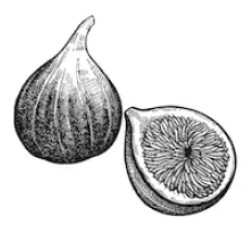
\includegraphics[width=1in,height=1.25in,clip,keepaspectratio]{fig1}}]{Michael Shell}
% Use $\backslash${\tt{begin\{IEEEbiography\}}} and then for the 1st argument use $\backslash${\tt{includegraphics}} to declare and link the author photo.
% Use the author name as the 3rd argument followed by the biography text.
% \end{IEEEbiography}

% \vspace{11pt}

% \bf{If you will not include a photo:}\vspace{-33pt}
% \begin{IEEEbiographynophoto}{John Doe}
% Use $\backslash${\tt{begin\{IEEEbiographynophoto\}}} and the author name as the argument followed by the biography text.
% \end{IEEEbiographynophoto}




% \vfill

\end{document}


